\documentclass[12pt]{article}

% chinese fonts
\usepackage{ctex}

% math fonts
\usepackage{amsmath}
\usepackage{amsthm}
\usepackage{amssymb}
\usepackage{bm}

% figures
\usepackage{tikz}
\usepackage{graphicx}
\graphicspath{{./figures/}}

% tables
\usepackage{tabularx}
\usepackage{booktabs}
\usepackage{multirow}
\usepackage[figuresright]{rotating}

\usepackage{enumerate}

% codes
\usepackage{listings}
\lstset{language     = Matlab,
        basicstyle   = \ttfamily,
        keywordstyle = \color{cyan},
        rulecolor    = \color{black},
        commentstyle = \color{green},
        keepspaces   = true,
        tabsize      = 4,
}

% hyperlinks
\usepackage{hyperref}
\hypersetup{
  breaklinks,
  colorlinks = true,
  citecolor  = blue,
  linkcolor  = red,
  urlcolor   = magenta,
}

% algorithms
\usepackage{algorithm}
\usepackage{algorithmic}

% bibliography
\usepackage[sort&compress,numbers]{natbib}

\include{macros}

\setlength{\oddsidemargin}{-0.25 in}
\setlength{\evensidemargin}{-0.25 in} 
\setlength{\topmargin}{-0.25in} 
\setlength{\textwidth}{7 in} 
\setlength{\textheight}{8.9 in}
\setlength{\headsep}{0.25 in} 
% \setlength{\parindent}{0 in}
\setlength{\parskip}{0.1 in}

\newcommand{\homework}[5]{
  \pagestyle{myheadings} 
  \thispagestyle{plain}
  \newpage
  \setcounter{page}{1} 
  \setcounter{section}{#5} 
  \noindent
  \begin{center}
    \framebox{ 
      \vbox{
        \vspace{2mm} 
        \hbox to 6.28in { {\bf
        THU-70250043-0,~Pattern~Recognition~(Spring 2021) \hfill Project: 1} }
        \vspace{6mm} 
        \hbox to 6.28in { {\Large \hfill #1 \hfill} }
        \vspace{6mm} 
        \hbox to 6.28in { {\it Lecturer: #2 \hfill} }
        \vspace{2mm} 
        \hbox to 6.28in { {\it \hspace{16mm} #3 \hfill} }
        \vspace{2mm} 
        \hbox to 6.28in { {\it Student: #4 \hfill} }
        \vspace{2mm} 
      } 
    }
  \end{center}
  \markboth{#1}{#1} 
  \vspace*{4mm} 
}

\begin{document}

\homework{商品图像检索}{Changshui Zhang
\hspace{4.2mm} {\tt zcs@mail.tsinghua.edu.cn}}{Hong Zhao \hspace{16mm} {\tt vzhao@tsinghua.edu.cn}}{Jingxuan Yang \hspace{10mm} {\tt yangjx20@mails.tsinghua.edu.cn}}{0}

\begin{abstract}

本文使用机器学习相关算法研究商品图像检索问题, 基于每个商品的图像信息和文本描述信息, 给定查询图片和文本, 在数据集中寻找与查询图片相似的图片, 输出全部相似图片的集合. 上述任务可以划分为三个子任务: 仅利用图像信息进行检索, 仅利用文本信息进行检索以及同时利用图像信息与文本信息进行检索. 针对上述三个子任务, 分别建立了 ResNet, ResNeXt, DenseNet, EfficientNet, NFNet, 图像模型 Ensemble 等 6 个图像模型, TF-IDF, BERT (2个), DistilBERT, SBERT (2个), 文本模型 Ensemble 等 7 个文本模型以及 TF-IDF 与 ResNet 取并集, SBERT 与 NFNet 取并集, TF-IDF 与 ResNet 度量层输出融合, SBERT 与 NFNet 度量层输出融合, 图像 Ensemble 与 文本 Ensemble 取并集等 5 个图像文本融合模型, 共计 18 个模型. 从机器学习的角度出发, 本文基于数据分布特性和嵌入空间特性提出了 Min2 最少两个原则以及 INB 迭代邻域混合两种模型改进方法, 这两种改进方法都使得原有模型的性能有了较大的提升. 针对数据集划分, 基于保证训练集, 验证集与测试集的数据保持相同分布的原则, 本文选择将数据集按组划分为 3:1:1 的三份, 分别作为训练集, 验证集与测试集. 针对评价指标, 本文选择精确率, 召回率以及 F1 分数三个指标, 计算方式为按行计算并取平均值. 所有的 18 个模型中, 以 F1 分数为评价依据, 性能最优的模型为 NFNet 模型 eca\_nfnet\_l0 与 SBERT 模型 paraphrase-xlm-r-multilingual-v1 进行度量层输出融合得到的模型, 其具体结果为 $\overline{F1}=0.888967,~\bar{R}=0.928442,~\bar{P}=0.893179$. 对于实验结果, 本文分析了模型超参数对性能的影响, 对单个模型得到了更优的模型超参数, 并且分析了特征的重要性, 发现文本特征对于商品图像检索任务更加重要. 本文还进行了错误分析, 案例分析以及实验结果的可视化分析, 对模型在不同数据集上的表现进行了全面深入和可视化的详细分析.

\textbf{关键词:}图像检索;文本检索;机器学习;深度学习;注意力机制;多模态学习

\end{abstract}

\newpage
\tableofcontents

\section{简介}

在如今的信息科技时代, 带有拍照功能的移动设备如手机、相机等得到了极大的普及和流行, 各种各样的图片和视频可以随时随地获得, 并借助互联网快速传播, 这种趋势使得网络上的数字图片和视频数据呈现出爆炸式的增长. 大量的数字图像信息给人们生产生活带来了许多便利的同时, 也给海量图像数据管理带来了挑战, 研究从海量的图像数据库中高效地查询到感兴趣的图像的技术变得越来越重要, 这种从图像数据库中查找给定图像的技术称为图像检索. 当前的图像检索方法按照数据有无标注可以划分为:监督、无监督、半监督、弱监督以及伪监督和自监督方法;按照模型主体结构又包括:自编码网络、孪生网络、对抗生成网络、注意力网络、循环神经网络等;按照特征的形式可以分为:二进制描述、实数特征描述以及聚合描述;按照检索方式又可以分为:基于文本的检索、基于内容的检索以及文本与图像多模态的检索三类方法 \cite{Dubey2020Decade}. 下面按照基于检索方式的分类对图像检索的发展历程与应用技术进行分析. 

基于文本的图像检索 (Text-based Image Retrieval, TBIR) 始于上世纪 70 年代 \cite{Hwang2012Medical,Alkhawlani2015Text}, TBIR 系统采用人工标注的方式对图像的内容进行文本关键词的标注, 并将标注存储, 然后根据用户输入的关键词来进行相关图像的检索, 如图 \ref{fig:TBIR} 所示. 这种方法在图像数据比较少时, 可以取得较好的检索效果, 但在图像数据量很大时, 人工标注方式不仅十分耗时, 而且人对图像的描述具有主观性, 不同人可能对同一张图像产生不同的描述, 从而造成文字描述图片的差异;另外, 图像包含丰富的信息, 有时很难用简短的关键词表示出图像中的内容, 使得检索效果难以尽如人意. 

\begin{figure}[htbp]
  \centering
  \includegraphics[width=12cm]{TBIR.png}
  \caption{基于文本的图像检索方法}
  \label{fig:TBIR}
\end{figure}

鉴于 TBIR 方法的局限性, 基于内容的图像检索 (Content-based Image Retrieval, CBIR) 技术被提出 \cite{Kato1992Database} . CBIR 用计算机技术对图像的内容进行分析, 将高维的数字图像矩阵表示成特征向量, 并将这些特征向量存入图像特征库中, 当用户输入查询图像时, 用相同的表示方法把查询图像表示成特征向量, 即查询向量, 然后依据相似性度量准则来计算查询向量与特征库中的每个特征向量之间的相似度, 最后将这些相似度进行大小排序, 按照从大到小的顺序输出对应的图像, 即返回的图像, 其完整过程如图 \ref{fig:CBIR} 所示. CBIR 将图像的内容表达交给了计算机进行自动处理, 克服了 TBIR 中依赖人工标注所面临的缺陷, 充分发挥了计算机长于计算的优势, 极大的提高了检索的效率, 使得图像检索在实际生产和生活中得到了广泛的应用.  

\begin{figure}[htbp]
  \centering
  \includegraphics[width=8cm]{CBIR.png}
  \caption{基于内容的图像检索方法}
  \label{fig:CBIR}
\end{figure}

对于 CBIR 方法来说需要解决三个问题:特征提取、相似度计算和特征压缩, 其中特征提取是 CBIR 技术中最主要的研究内容 \cite{Smeulders2000Content}. 通常检索一张图片的相似图片需要在庞大的数据库内进行检索, 因此检索效率就和检索准确率一样是非常重要的指标, 而提升检索效率的关键就在于生成比较小但是又足够丰富的图像特征. 图像特征提取主要包含特征工程和特征学习两个阶段 \cite{Chen2021Deep}. 在特征工程阶段, 早期的 CBIR 技术大多数使用全局视觉特征来进行图像的表示. 这种特征描述方式比较简洁, 使用者可以很方便高效的进行图像检索. 但是, 由于这种方法提取的是图像低层视觉特征, 当遇到外界因素的干扰, 如光照强度、遮挡、形变等恶劣条件时, 此时无法准确提取到图像的有效特征. 后来, 研究人员设计了一系列局部特征提取的方法, 这些方法使用一组特征来描述图像, 比如 HOG (Histograms of Oriented Gradients) \cite{Dalal2005Histograms}、SIFT (Scale Invariant Feature Transform) \cite{Lowe1999Object}、SURF (Speeded up Robust  Features) \cite{Bay2006Surf}、BRIEF (Binary 
Robust Independent Elementary Features) \cite{Calonder2010Brief}、ORB (Oriented FAST and Rotated BRIEF) \cite{Rublee2011Orb}、Harris 角点 (Harris Corner) \cite{Harris1988Combined} 等, 并以此为基础通过不同的编码方式构建图像的全局描述, 具有代表性的工作有词袋模型 (Bag of Words, BoW) \cite{Sivic2008Efficient}、局部特征聚合描述符 (Vector of Locally Aggregated Descriptors, VLAD) \cite{Jegou2010Aggregating} 以及 Fisher 向量 (Fisher Vector, FV) \cite{Perronnin2007Fisher} 等. 早期主要通过手工进行特征提取的 CBIR 系统, 虽然在检索上取到一定的效果, 但由于受到人们理解图像特征存在“语义鸿沟”及不能准确的对图像特征相似度的判别等问题, 导致检索的准确度比较低, 从而限制了基于内容图像检索的发展. 

随着 2012 年 ImageNet 和深度卷积神经网络 (Deep Convolutional Neural Network, DCNN) AlexNet \cite{Krizhevsky2012Imagenet} 的出现, 特征提取的研究开始进入特征学习的阶段. DCNN 可以直接从数据中学习到非常有效的位于不同抽象层次的图像特征, 从而给图像检索领域带来了巨大的进步. 深度卷积神经网络对图像检索的改进主要从网络层面和特征层面入手, 在网络层面可以改进网络结构和微调网络参数, 在特征层面可以进行深度特征提取和深度特征增强. DCNN 的层次结构和广泛的参数化使其在各种各样的计算机视觉任务中获得了成功. 对于图像检索, 有四种主要作为特征提取网络的模型, 包括 AlexNet \cite{Krizhevsky2012Imagenet}、VGGNet \cite{Simonyan2014Very}、GoogLeNet \cite{Szegedy2015Going} 和 ResNet \cite{He2016Deep}. 

图像检索中必须克服的另一个难点是:随着图像数据规模的急剧增长以及特征索引库中高维度特征数据, 当前基于最近邻检索方法难以获得可接受的响应时间. 针对这个问题, 近似最近邻算法 (Approximate Nearest Neighbor, ANN) \cite{Arya1998Optimal} 中的哈希方法可以很好的解决大规模图像特征向量的存储和索引问题, 它的核心思想是通过将车辆图像的高维特征投影为低维度的二值编码, 得到的二值编码与原有的高维特征向量保持一致的对应关系. 常用的哈希方法包括有监督和无监督两种 \cite{Wang2017Survey}. 无监督方法在构造二值编码的过程中只使用数据项不使用标签, 代表性方法有 LSH (Locality Sensitive Hashing) \cite{Charikar2002Similarity}、ITQ (Iterative Quantization) \cite{Gong2012Iterative}、SH (Spectral Hashing) \cite{Weiss2008Spectral} 等. 有监督哈希方式是使用标签信息参与二值编码的构建, 其中最具有代表性的方法有:SDH (Supervised Discrete Hashing) \cite{Shen2015Supervised}、KSH (Kernel-based Supervised Hashing) \cite{Liu2012Supervised}、和 BRE (Binary Reconstruction Embeddings) \cite{Kulis2009Learning} 等. 

为了进一步提升检索效果, 人们开始进行文本与图像之间的跨模态检索或联合文本与图像的多模态检索. 现有的大多数图像文本检索方法要么将完整的图像和完整的句子嵌入到一个共享空间中, 要么考虑局部片段之间的潜在对应关系, 还有一些方法采用注意力机制来关注最重要的局部区域. Vo 等人对输入图像加上了一些描述文本, 该文本指定了对输入图像要做出的修改, 而后提出了一种新的基于残差连接的图像与文本相结合的方法, 寻找出与修改后图片相似的图像 \cite{Vo2019Composing}. 图像文本双向检索作为一种典型的跨模式检索问题, 在很大程度上依赖于图像与文本的联合嵌入学习和相似性度量. Zhang 等人提出了一个统一的上下文感知注意网络 (Context-Aware Attention Network, CAAN), 它通过聚合全局上下文选择性地关注关键的图片局部区域和某个特定单词 \cite{Zhang2020Context}. Wang 等人针对联合嵌入空间中图像与文本之间的交互作用, 提出了跨模态自适应消息传递 (Cross-Modal Adaptive Message Passing, CAMP) 模型, 它可以自适应地控制信息流, 以实现跨模态的消息传递 \cite{Wang2019CAMP}. Chen 等人根据查询意图引入注意力机制来自适应地平衡不同模式的重要性, 提出了一种新的注意引导多模态相关 (Attention guided Multi-modal Correlation, AMC) 学习方法, 该方法由注意网络内部和注意网络之间的联合学习层次构成 \cite{Chen2017AMC}. 为了提高模型应用部署效率, 基于 BERT \cite{Devlin2018BERT} 的预训练模型如 ViLBERT (Vision-and-Language BERT) \cite{Lu2019ViLBERT}、VisualBERT \cite{Su2019VL} 和 VL-BERT (Visual-Linguistic BERT) \cite{Li2019VisualBERT} 等被提出用来预学习图像和文本联合嵌入空间的特征. 

图像检索还需要解决数据长尾分布的问题, 现实世界的数据集总是带有长尾的偏态分布 \cite{Van2017Devil}, 即少数类(又称头部类)占据了大部分数据, 而大多数类(又称尾部类)很少有样本. 此外, 近年来计算机视觉界构建和发布了越来越多反映现实规律的长尾数据集, 如 iNat2017 (iNaturalist Classification and Detection Dataset) \cite{Van2018iNaturalist}、LVIS (Large Vocabulary Instance Segmentation Dataset) \cite{Gupta2019LVIS} 和 RPC (Retail Product Checkout Dataset) \cite{Wei2019RPC}. 在处理这些长尾分布的数据时, 由于极端的类别分布不平衡问题, 深度学习方法无法获得很好的辨识精度. 
% 类重平衡策略(如重加权和重抽样)是解决长尾问题中极端不平衡问题的重要而有效的方法. 这些再平衡方法能够显著地促进深层网络的分类器学习, 从而获得令人满意的识别精度, 但同时也会在一定程度上意外地损害所学深层特征的表征能力. 
Zhou 等人提出了一个统一的双边分支网络 (Bilateral-Branch Network, BBN) 来同时处理表示学习和分类器学习, 其中每个分支分别执行自己的任务, 并且配备了一种新的累积学习策略, 即先学习通用模式, 然后逐渐关注尾部数据 \cite{Zhou2020BBN}. Schroeder 等人提出了一种基于场景图嵌入的图像检索方法, 研究了如何将从场景图派生的可视关系用作结构化查询 \cite{Schroeder2020Structured}. Zhou 等人针对长尾问题, 提出了一种新的基于侧边信息的大规模视觉识别协同训练系统 (Side Information Based Large Scale Visual Recognition Co-Training, SICoT), 引入了一个双线性词注意模块, 在有噪声的边信息上构造一个语义嵌入, 然后设计了一种基于视觉特征和语义嵌入的协同训练方案, 以端到端的方式将知识从训练数据丰富的头部类转移到训练数据较少的尾部类 \cite{Zhou2020Large}. 

图像检索还涉及到鲁棒性的问题, 由于噪声、分辨率、压缩和光照等多种失真, 计算机视觉算法在摄像机捕获图像上的应用性能会下降. 为了保证视觉分析算法的可靠, 有必要确保计算机视觉算法在处理这些失真图像时的鲁棒性. Somasundaran 等人通过对图像检索问题的研究, 重点讨论了鲁棒性问题的一个具体实例, 考虑了图像增强算法的设计, 以确保在由于噪声和低分辨率引起的失真情况下检索算法的鲁棒性 \cite{Somasundaran2020Robust}.  Humenberger 等人则提出了一种通用的视觉定位方法, 它基于鲁棒图像检索进行粗略的摄像机姿态估计, 并且基于鲁棒局部特征进行精确的姿态细化 \cite{Humenberger2020Robust}. 

\paragraph{本文主要贡献} 商品图像检索任务可以划分为三个子任务: 仅利用图像信息进行检索, 仅利用文本信息进行检索以及同时利用图像信息与文本信息进行检索. 针对上述三个子任务, 本文分别建立了 ResNet, ResNeXt, DenseNet, EfficientNet, NFNet, 图像模型 Ensemble 等 6 个图像模型, TF-IDF, BERT (2个), DistilBERT, SBERT (2个), 文本模型 Ensemble 等 7 个文本模型以及 TF-IDF 与 ResNet 取并集, SBERT 与 NFNet 取并集, TF-IDF 与 ResNet 度量层输出融合, SBERT 与 NFNet 度量层输出融合, 图像 Ensemble 与 文本 Ensemble 取并集等 5 个图像文本融合模型, 共计 18 个模型. 本文基于数据分布特性和嵌入空间特性分别提出了 Min2 最少两个原则以及 INB 迭代邻域混合两种模型改进方法, 这两种改进方法都使得原有模型的性能有了较大的提升.

\section{任务定义}

\subsection{仅利用图像信息}

输入为图像 $\vx\in\reals^{C_{\text{in}}\times H\times W}$, 其中 $C_{\text{in}}$ 表示通道, $H$ 表示图像高度, $W$ 表示图像深度, 令 $\text{id}_{\vx}$ 表示图像 $\vx$ 的 posting\_id. 通过神经网络等算法以图像为输入得到嵌入向量 $\vy_{\vx}\in\reals^{p}$, 对得到的嵌入向量进行基于余弦距离的近邻算法可以得到相似图像, 输出为关于输入图像相似图像的 posting\_id 集合 $S_{\vx}=\{\id_{\vx},\id_{\vx_1},\id_{\vx_2},\dots\}$.

除可以使用单个模型进行处理之外, 还可以把多个模型进行 Ensemble, 这时模型输出的结果为 Ensemble 后的模型得到的关于输入图像相似图像的 posting\_id 集合 $S_{\vx}=\{\id_{\vx},\id_{\vx_1},\id_{\vx_2},\dots\}$.

\subsection{仅利用文本信息}

输入为文本 $d$, 具体而言是指图片 $\vx$ 的标题文本, 通过某些文本处理方法得到文本的嵌入向量 $\vy_d\in\reals^{q}$. 通过对得到的嵌入向量进行基于某种距离的近邻算法可以得到相似图像, 输出为关于输入图像相似图像的 posting\_id 集合 $S_{d}=\{\id_{\vx},\id_{\vxt_1},\id_{\vxt_2},\dots\}$. 

与仅利用图像信息类似, 除可以使用单个模型对文本信息进行处理之外, 也可以把多个模型进行 Ensemble, 这时模型输出的结果为 Ensemble 后的模型得到的关于输入图像相似图像的 posting\_id 集合 $S_d=\{\id_{\vx},\id_{\vx_1},\id_{\vx_2},\dots\}$.

\subsection{同时利用图像与文本信息}

输入为图像 $\vx\in\reals^{C_{\text{in}}\times H\times W}$, 其中 $C_{\text{in}}$ 表示通道, $H$ 表示图像高度, $W$ 表示图像深度, 以及相应的图像标题文本 $d$. 分别对图像和文本进行处理得到相应的嵌入向量 $\vy_{\vx}\in\reals^{p}$ 和 $\vy_{d}\in\reals^{q}$, 通过对得到的嵌入向量分别进行基于某种距离的近邻算法可以得到相似图像的 posting\_id 集合 $S_{\vx}=\{\id_{\vx},\id_{\vx_1},\id_{\vx_2},\dots\}$ 与 $S_{d}=\{\id_{\vx},\id_{\vxt_1},\id_{\vxt_2},\dots\}$, 最终输出为两个集合的并集
\begin{equation}
  S = S_{\vx}\cup S_{d}
\end{equation}

除了使用并集的方法处理文本模型和图像模型外, 还可以对文本模型和图像模型进行 Ensemble, 具体而言可以选择多个模型的度量层输出进行融合, 这时模型输出的结果为 Ensemble 后的模型得到的关于输入图像相似图像的 posting\_id 集合 $S=\{\id_{\vx},\id_{\vx_1},\id_{\vx_2},\dots\}$.

\section{数据整理}

数据集来自 Kaggle 竞赛 \href{https://www.kaggle.com/c/shopee-product-matching/overview}{Shopee - Price Match Guarantee}, 包含 \verb|train.csv| 和 \verb|test.csv| 两个 \verb|csv| 文件以及 \verb|train_images/| 和 \verb|test_images/| 两个图像文件夹. 

\verb|train.csv| 文件包含 34250 行数据, 其前 5 行如表 \ref{tab:train_csv_5} 所示, 第一列为索引, 第二列为每张图片独特的识别 id, 第三列为图片文件名, 第四列为图片感知哈希值, 第五列为图像的标题, 主要为印尼语和部分英语, 第六列为图像的标签, 相同的标签表示图像为同一个类别, 表格中没有缺失数据. \verb|train_images/| 文件夹包含 32412 张图片, 图片的文件名与 \verb|train.csv| 中的 image 列相对应.

\begin{table}[htbp]
  \footnotesize
  \centering
  \caption{train.csv 数据示例}
  \label{tab:train_csv_5}
  \begin{tabular}{p{0.5cm}p{2.5cm}p{3cm}p{2.7cm}p{4cm}p{1.9cm}}
    \toprule
    index & posting\_id       & image                                & image\_phash     & title                                                                                              & label\_group \\
    \midrule
    0 & train\_129225211  & 0000a68812bc7e98c 42888dfb1c07da0.jpg & 94974f937d4c2433 & Paper Bag Victoria Secret                                                                          & 249114794    \\
    1 & train\_3386243561 & 00039780dfc94d01db 8676fe789ecd05.jpg & af3f9460c2838f0f & Double Tape 3M VHB 12 mm x 4,5 m ORIGINAL / DOUBLE FOAM TAPE                                       & 2937985045   \\
    2 & train\_2288590299 & 000a190fdd715a2a36 faed16e2c65df7.jpg & b94cb00ed3e50f78 & Maling TTS Canned Pork Luncheon Meat 397 gr                                                        & 2395904891   \\
    3 & train\_2406599165 & 00117e4fc239b1b641 ff08340b429633.jpg & 8514fc58eafea283 & Daster Batik Lengan pendek - Motif Acak / Campur - Leher Kancing (DPT001-00) Batik karakter Alhadi & 4093212188   \\
    4 & train\_3369186413 & 00136d1cf4edede020 3f32f05f660588.jpg & a6f319f924ad708c & Nescafe \textbackslash{}xc3\textbackslash{}x89clair Latte 220ml                                    & 3648931069  \\
    \bottomrule
  \end{tabular}
\end{table}

计算 \verb|train.csv| 每一列非重复的元素个数, 如表 \ref{tab:unique_values} 所示. 

\begin{table}[htbp]
  \small
  \centering
  \caption{train.csv 每列非重复元素个数}
  \label{tab:unique_values}
  \begin{tabular}{cc}
    \toprule
    column & number of unique values \\
    \midrule
    posting\_id & 34250 \\
    image & 32412 \\
    image\_phash & 28735 \\
    title & 33117 \\
    label\_group & 11014 \\
    \bottomrule
  \end{tabular}
\end{table}

由表可知图片类别标签共有 11014 类, 显然图像文件名, 图像感知哈希以及图像标题都存在重复的数据, 所以我们可以进行数据清洗. 通过编写以下代码进行数据清洗, 查找 (image, image\_phash, title) 均相同的数据行 

\verb|df_train.drop_duplicates(["image", "image_phash", "title"], inplace=True)|, 

但是最终数据却没有一行被删除, 由此可知, 虽然单独来看图像文件名, 图像感知哈希以及图像标题都有重复的存在, 但是三者同时重复的数据项却并不存在, 因此并不需要进行数据清洗.

下面研究图像标签的分布情况, 画出图像标签的分布如图 \ref{fig:dist_label_group} 所示, 可以看出大部分标签包含 10 张以下图片, 只有少数的标签包含 50 张左右的图片.

\begin{figure}[htbp]
  \centering
  \includegraphics[width=12cm]{dist_label_group.png}
  \caption{图像标签的分布}
  \label{fig:dist_label_group}
\end{figure}

相同类别图像个数最多的 10 个类别及其图像个数如表 \ref{tab:most_frequent_label_groups} 所示, 其中前七个类别包含的图像数量都多达 51 个.

\begin{table}[htbp]
  \small
  \centering
  \caption{Top 10 最频繁出现的图像类别}
  \label{tab:most_frequent_label_groups}
  \begin{tabular}{ccc}
    \toprule
    index  & label\_group & number of images \\
    \midrule
    0 & 1141798720  & 51               \\
    1 & 3113678103  & 51               \\
    2 & 562358068   & 51               \\
    3 & 3627744656  & 51               \\
    4 & 994676122   & 51               \\
    5 & 1163569239  & 51               \\
    6 & 159351600   & 51               \\
    7 & 3206118280  & 49               \\
    8 & 1166650192  & 46               \\
    9 & 1733221456  & 46    \\
    \bottomrule          
  \end{tabular}
\end{table}

这些类别中, 排在最前面两个类别 1141798720 以及 3113678103 内包含的图像分别如图 \ref{fig:label_1141798720} 和 \ref{fig:label_3113678103} 所示, 可以看出图中商品分别为护肤品和水管软头.

\begin{figure}[htbp]
  \centering
  \begin{minipage}[t]{0.48\textwidth}
    \centering
    \includegraphics[width=8cm]{label_1141798720.jpg}
    \caption{类别 1141798720 包含的图像}
    \label{fig:label_1141798720}
  \end{minipage}
  \begin{minipage}[t]{0.48\textwidth}
    \centering
    \includegraphics[width=8cm]{label_3113678103.jpg}
    \caption{类别 3113678103 包含的图像}
    \label{fig:label_3113678103}
  \end{minipage}
\end{figure}

下面研究图像标题文本的分布情况, 画出标题文本的分布如图 \ref{fig:dist_title} 所示, 可以看出大部分标题文本包含 2 张以下图片, 只有少数的标题文本包含 8 张左右的图片.

\begin{figure}[htbp]
  \centering
  \includegraphics[width=14cm]{dist_title.png}
  \caption{图像标题文本的分布}
  \label{fig:dist_title}
\end{figure}

相同标题文本个数最多的 10 个类别及其标题个数如表 \ref{tab:most_frequent_title} 所示, 与图像标签相比, 相同标题文本的图像个数要少了很多, 最多的也仅有 9 个.

\begin{table}[htbp]
  \centering
  \footnotesize
  \caption{Top 10 最频繁出现的标题文本}
  \label{tab:most_frequent_title}
  \begin{tabular}{p{0.8cm}p{9cm}p{3cm}}
    \toprule
    index & title                                                                                                & number of images \\
    \midrule
    0     & Koko syubbanul muslimin koko azzahir koko baju                                                       & 9                \\
    1     & Baju Koko Pria Gus Azmi Syubbanul Muslimin Kombinasi Hadroh Azzahir Hilw HO187 KEMEJA KOKO PRIA BAJU & 8                \\
    2     & 100 Pcs Ikat Rambut Karet Polos Elastis Gaya Korea untuk Wanita                                      & 6                \\
    3     & Viva Air Mawar                                                                                       & 6                \\
    4     & Monde Boromon Cookies 1 tahun+ 120gr                                                                 & 6                \\
    5     & Emina Glossy Stain                                                                                   & 6                \\
    6     & Wardah Everyday Fruity Sheer Lip Balm Strawberry 4g                                                  & 5                \\
    7     & Avoskin Miraculous Retinol Toner                                                                     & 5                \\
    8     & Shannen lipstik shanen creamy lip paint                                                              & 5                \\
    9     & Herborist Lulur Tradisional Bali 100gr                                                               & 5               \\
    \bottomrule
  \end{tabular}
\end{table}

这些标题中, 排在最前面两个标题包含的图像分别如图 \ref{fig:title_Kok} 和 \ref{fig:title_Baj} 所示, 可以看出图中商品都是男士衬衫.

\begin{figure}[htbp]
  \centering
  \begin{minipage}[t]{0.48\textwidth}
    \centering
    \includegraphics[width=8cm]{title_Kok.jpg}
    \caption{标题 Koko syubbanul ... 包含的图像}
    \label{fig:title_Kok}
  \end{minipage}
  \begin{minipage}[t]{0.48\textwidth}
    \centering
    \includegraphics[width=8cm]{title_Baj.jpg}
    \caption{标题 Baju Koko Pria ... 包含的图像}
    \label{fig:title_Baj}
  \end{minipage}
\end{figure}

标题文本长度的分布如图 \ref{fig:dist_title_length} 所示, 可以看出标题文本长度大多在 100 词以下, 但有少部分标题文本长度达到了 350 词左右.

\begin{figure}[htbp]
  \centering
  \includegraphics[width=14cm]{dist_title_length.png}
  \caption{图像标题文本长度的分布}
  \label{fig:dist_title_length}
\end{figure}

对全部的标题文本做出词云, 如图 \ref{fig:word_cloud} 所示, 可以看出 Double, Tape, Bag, Paper 等词出现的频率较高.

\begin{figure}[htbp]
  \centering
  \includegraphics[width=10cm]{word_cloud.jpg}
  \caption{标题词云图}
  \label{fig:word_cloud}
\end{figure}

下面研究图像感知哈希的分布情况, 画出感知哈希的分布如图 \ref{fig:dist_image_phash} 所示, 可以看出大部分感知哈希包含 5 张以下图片, 只有少数的感知哈希包含 25 张左右的图片.

\begin{figure}[htbp]
  \centering
  \includegraphics[width=14cm]{dist_image_phash.png}
  \caption{图像感知哈希的分布}
  \label{fig:dist_image_phash}
\end{figure}

\section{方法设计}

\subsection{仅利用图像信息}

针对图像信息, 本文采用 ResNet, ResNeXt, DenseNet, EfficientNet, 以及 NFNet 进行处理, 最后对这五个模型进行 Ensemble.

\subsubsection{ResNet}

% https://www.jianshu.com/p/93990a641066

ResNet (Residual Neural Network) \cite{He2016Deep} 是残差神经网络, 主要解决的是深度神经网络的退化问题. 我们知道, 对浅层网络逐渐叠加层数, 模型在训练集和测试集上的性能会变好, 因为模型复杂度更高了, 表达能力更强了, 可以对潜在的映射关系拟合得更好. 而退化指的是, 给网络叠加更多的层后, 性能却快速下降的情况. 

ResNet 从调整模型结构入手, 探求更好的模型结构. 将堆叠的几层称之为一个块, 对于某个块, 其可以拟合的函数为 $F(x)$, 如果期望的潜在映射为 $H(x)$, 与其让 $F(x)$ 直接学习潜在的映射, 不如去学习残差 $H(x)-x$, 即 $F(x)\triangleq H(x)-x$, 这样原本的前向路径上就变成了 $F(x)+x$, 用 $F(x)+x$ 来拟合 $H(x)$. 这样可能更易于优化, 因为相比于让 $F(x)$ 学习成恒等映射, 让 $F(x)$ 学习成 0 要更加容易, 后者通过 $\ell_2$ 正则就可以实现. 这样, 对于冗余的块, 只需 $F(x)\rightarrow 0$ 就可以得到恒等映射, 性能不减. 

$F(x)+x$ 构成的块称为残差块, 如图 \ref{fig:resnet} 所示, 多个相似的残差块串联构成残差网络. 一个残差块有两条路径 $F(x)$ 和 $x$, $F(x)$ 路径拟合残差, 不妨称之为残差路径, $x$ 路径为恒等映射, 称之为 shortcut. 

\begin{figure}[htbp]
  \centering
  \includegraphics[width=10cm]{block.pdf}
  \caption{ResNet 残差块}
  \label{fig:resnet}
\end{figure}

残差路径可以大致分成两种, 一种有瓶颈 (bottleneck) 结构, 即图 \ref{fig:resnet_function} 右中的 $1\times1$ 卷积层, 用于先降维再升维, 主要出于降低计算复杂度的现实考虑, 称之为瓶颈块, 另一种没有瓶颈结构, 如图 \ref{fig:resnet_function} 左所示, 称之为基本块. 

\begin{figure}[htbp]
  \centering
  \includegraphics[width=12cm]{block_deeper.pdf}
  \caption{ResNet 残差路径}
  \label{fig:resnet_function}
\end{figure}

Shortcut 路径大致也可以分成两种 \cite{Zhang2020Dive}, 取决于残差路径是否改变了特征映射的数量和尺寸, 一种是将输入 $x$ 原封不动地输出, 另一种则需要经过 $1\times1$ 卷积来升维或降采样, 主要作用是将输出与 $F(x)$ 路径的输出保持形状一致, 对网络性能的提升并不明显, 两种结构如图 \ref{fig:resnet_shortcut} 所示.

\begin{figure}[htbp]
  \centering
  \includegraphics[width=12cm]{resnet_shortcut.png}
  \caption{ResNet shortcut 路径}
  \label{fig:resnet_shortcut}
\end{figure}

\subsubsection{ResNeXt}

% https://blog.csdn.net/u014380165/article/details/71667916

ResNeXt \cite{Xie2017Aggregated} 是 ResNet 的改进版本, 指的是 Next ResNet. ResNeXt 提出的主要原因在于传统提高模型的准确率的方法都是加深或加宽网络, 但是随着超参数数量的增加, 网络设计的难度和计算开销也会增加. 得益于子模块的拓扑结构, ResNeXt 可以在不增加参数复杂度的前提下提高准确率, 同时还减少了超参数的数量. 

ResNeXt 是 ResNet 和 Inception 的结合体, 不同于 Inception 的是, ResNeXt 不需要人工设计复杂的 Inception 结构细节, 而是每一个分支都采用相同的拓扑结构. ResNeXt 的本质是分组卷积 (Group Convolution), 通过变量基数 (Cardinality) 来控制组的数量. 组卷积是普通卷积和深度可分离卷积的一个折中方案, 即每个分支产生的特征图谱的通道数为 $n(n>1)$.

Inception 是一个非常明显的分割变换合并结构, 其不同分支的不同拓扑结构的特征有非常刻意的人工雕琢的痕迹, 而往往调整 Inception 的内部结构对应着大量的超参数, 这些超参数调整起来是非常困难的. ResNeXt 的每个结构使用相同的拓扑结构, 那么这时候的 Inception 表示为
\begin{equation}
  \Fc(\vx)=\sum_{i=1}^C\mathcal{T}_i(\vx)
\end{equation}

其中 $C$ 是基数 (Cardinality),  $\mathcal{T}_i$ 是任意的变换, 例如一系列的卷积操作等. 图 \ref{fig:resnext_inception} 便是一个简化的 Inception, 其 $\mathcal{T}_i$ 是由连续的卷积组成 ($1\times1\to3\times3\to1\times1$).

\begin{figure}[htbp]
  \centering
  \includegraphics[width=9cm]{resnext_inception.pdf}
  \caption{ResNeXt Inception 示例}
  \label{fig:resnext_inception}
\end{figure}

结合残差网络, 我们便可以得到完整的 ResNeXt, 也就是在简化 Inception 中添加一条 shortcut, 如图 \ref{fig:resnext_residual} 所示, 表示为
\begin{equation}
  \vy=\vx+\sum_{i=1}^C\mathcal{T}_i(\vx)
\end{equation}

\begin{figure}[htbp]
  \centering
  \includegraphics[width=10cm]{resnext_residual.pdf}
  \caption{ResNeXt 结构}
  \label{fig:resnext_residual}
\end{figure}

\subsubsection{DenseNet}

% https://zhuanlan.zhihu.com/p/43057737

DenseNet (Dense Convolutional Network) \cite{Huang2017Densely} 脱离了加深网络层数 (ResNet) 和加宽网络结构 (Inception) 来提升网络性能的定式思维, 从特征的角度考虑, 通过特征重用和旁路 (Bypass) 设置, 既大幅度减少了网络的参数量, 又在一定程度上缓解了梯度消失问题的产生.

DenseNet 作为另一种拥有较深层数的卷积神经网络, 具有如下优点:

(1) 相比 ResNet 拥有更少的参数数量.

(2) 旁路加强了特征的重用.

(3) 网络更易于训练, 并具有一定的正则效果.

(4) 缓解了梯度消失和模型退化的问题.

假设输入为一个图片 $\mx_0$ , 经过一个 $L$ 层的神经网络, 其中第 $i$ 层的非线性变换记为 $H_i(\cdot)$, $H_i(\cdot)$ 可以是多种函数操作的累加如 BN, ReLU, Pooling 或 Conv 等. 第 $i$ 层的特征输出记作 $\mx_i$. 传统卷积前馈神经网络将第 $i$ 层的输出 $\mx_i$ 作为 $i+1$ 层的输入, 可以写作 $\mx_i=H_i(\mx_{i-1})$. ResNet 增加了旁路连接, 可以写作
\begin{equation}
  \mx_i=H_i(\mx_{i-1})+\mx_{i-1}
\end{equation}

ResNet 的一个最主要的优势便是梯度可以流经恒等函数来到达靠前的层, 但恒等映射和非线性变换输出的叠加方式是相加, 这在一定程度上破坏了网络中的信息流. 为了进一步优化信息流的传播, DenseNet 提出了如图 \ref{fig:dense_block} 所示的网络结构.
\begin{figure}[htbp]
  \centering
  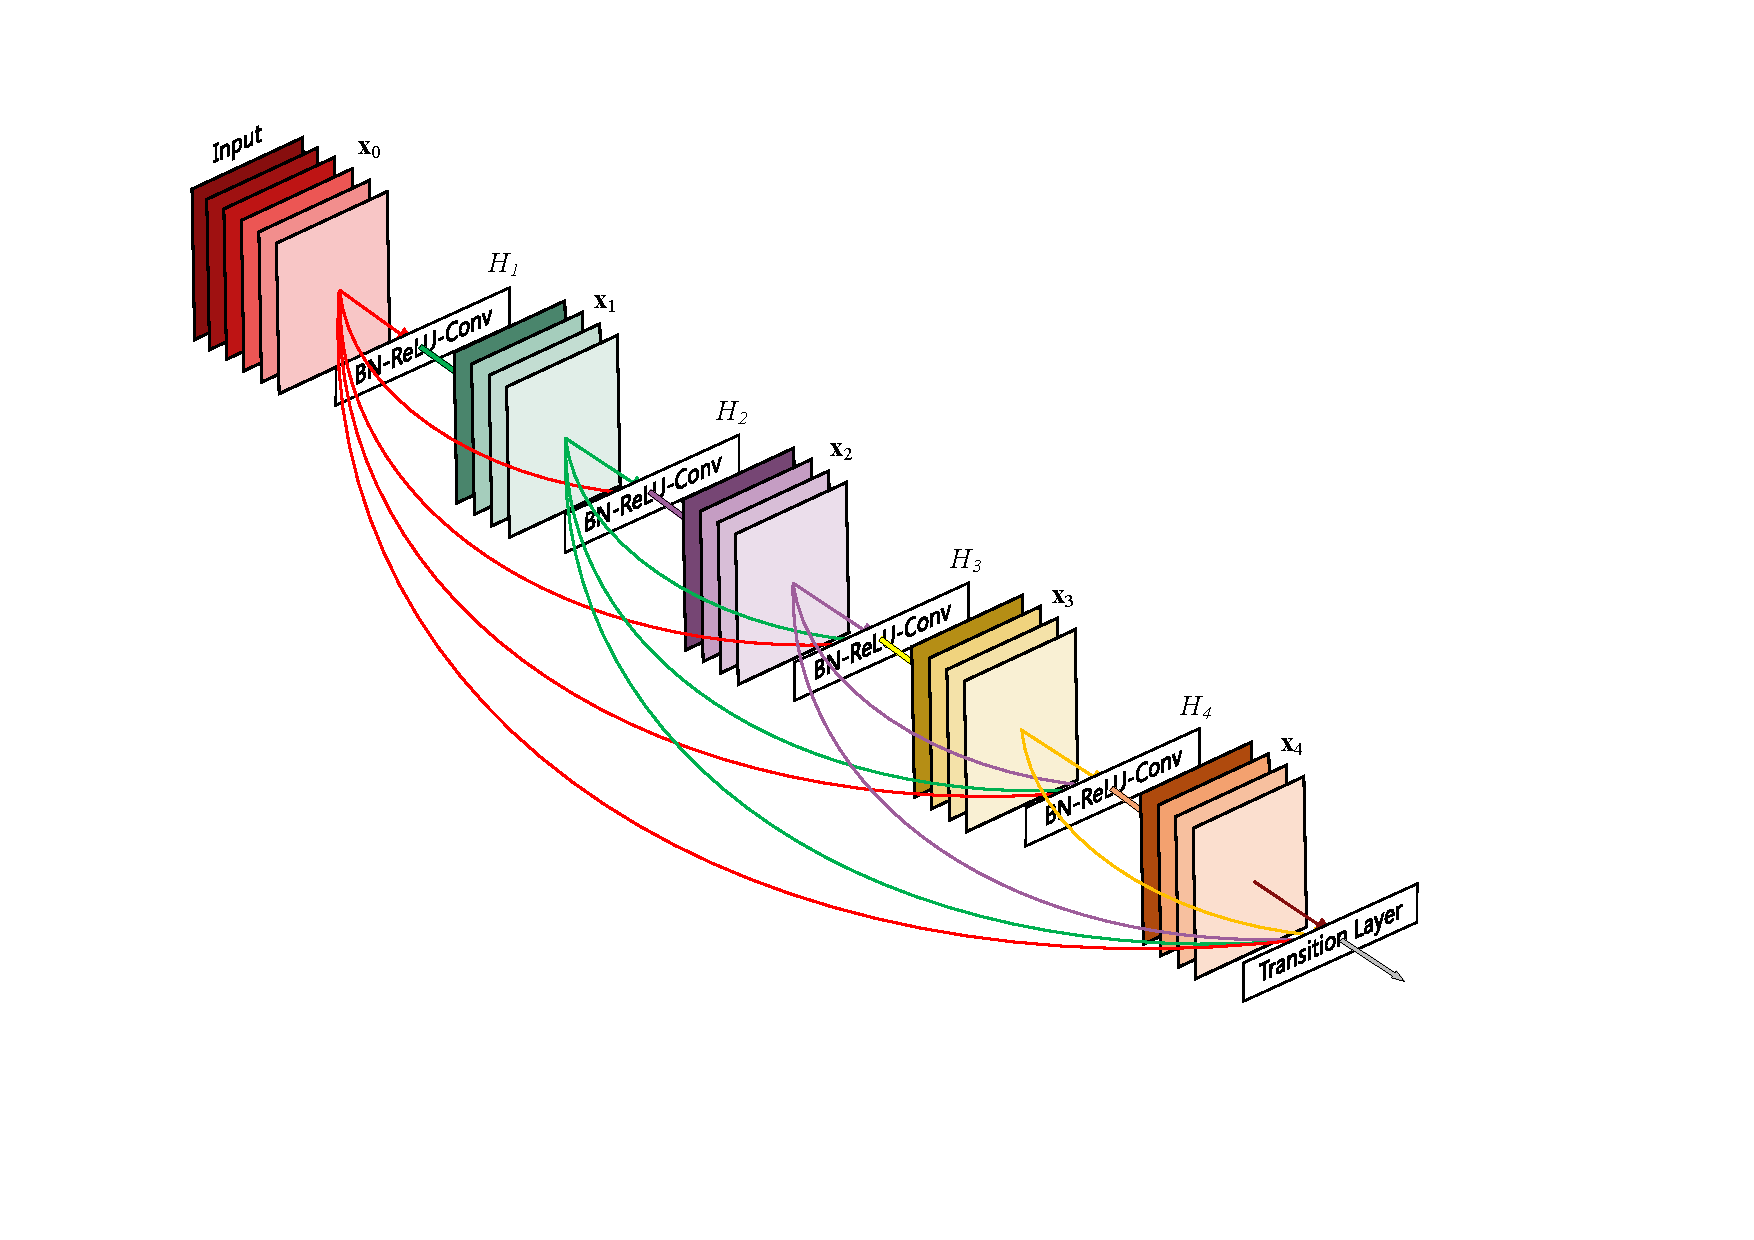
\includegraphics[width=12cm]{denseBlock.pdf}
  \caption{DenseNet 5 层网络块}
  \label{fig:dense_block}
\end{figure}

如图所示, 第 $i$ 层的输入不仅与 $i-1$ 层的输出相关, 还与所有之前层的输出有关, 记作
\begin{equation}
  \mx_i=H_i([\mx_{0},\mx_{1},\dots,\mx_{i-1}])
\end{equation}

其中 $[\mx_{0},\mx_{1},\dots,\mx_{i-1}]$ 代表拼接, 即将 $\mx_0$ 到 $\mx_{i-1}$ 层的所有输出特征按通道组合在一起, 这里所用到的非线性变换 $H_i(\cdot)$ 为 BN, ReLU 和 $3\times3$ 卷积的组合.

在 DenseNet 中需要对不同层的输出特征进行拼接操作, 所以需要不同层的输出特征保持相同的大小, 这就限制了网络中下采样的实现. 为了使用下采样, 将 DenseNet 分为多个网络块, 如图 \ref{fig:dense_net} 所示. 在同一个网络块中要求输出特征保持相同大小, 在不同网络块之间设置变换层实现下采样.

\begin{figure}[htbp]
  \centering
  \includegraphics[width=17cm]{denseNet.pdf}
  \caption{具有三个网络块的 DenseNet}
  \label{fig:dense_net}
\end{figure}

在网络块中, 假设每一个非线性变换 $H$ 的输出为 $k$ 个输出特征, 那么第 $i$ 层网络的输入便为 $k_0+(i-1)k$, 这里我们可以看到 DenseNet 和现有网络的一个主要的不同点: DenseNet 可以接受较少的特征图数量作为网络层的输出, 原因就是在同一个网络块中的每一层都与之前所有层相关联, 如果我们把特征看作是一个网络块的全局状态, 那么每一层的训练目标便是通过现有的全局状态, 判断需要添加给全局状态的更新值. 因而每个网络层的输出特征数量 $k$ 又称为生长率, 同样决定着每一层需要给全局状态更新的信息的多少.

\subsubsection{EfficientNet}

% https://www.jianshu.com/p/2ac06d97a830

EfficientNet \cite{Tan2019Efficientnet} 提出了一种多维度混合的模型放缩方法. 模型放缩的几个常用维度是网络深度、网络宽度和图像分辨率, 以前的模型多是放大其中的一个维度以达到更高的准确率, 比如 ResNet-18 到 ResNet-152 是通过增加网络深度的方法来提高准确率. EfficientNet 则从一个高度去审视这些放缩维度, 认为这三个维度之间是互相影响的并探索出了三者之间最好的组合, 该网络的表现如 \ref{fig:effnet_params} 所示.

\begin{figure}[htbp]
  \centering
  \includegraphics[width=10cm]{effnet_params.pdf}
  \caption{EfficientNet 与其他模型对比}
  \label{fig:effnet_params}
\end{figure}

将整个卷积网络称为 $\Nc$, 它的第 $i$ 个卷积层可以看作是下面的函数映射
\begin{equation}
  Y_i = \Fc_i(X_i)
\end{equation}

$Y_i$ 为输出张量, $X_i$ 为输入张量, 设其维度为 $\langle H_i, W_i, C_i \rangle$, 那么整个卷积网络由 $k$ 个卷积层组成, 可以表示为
\begin{equation}
  \Nc = \Fc_k \odot \dots \odot  \Fc_2 \odot \Fc_1 (X_1) = \bigodot_{j=1,2,\dots,k} \Fc_j (X_1)
\end{equation}

实际中, 通常将多个结构相同的卷积层称为一个阶段 (Stage), 例如 ResNet 可以分为 5 个阶段, 每个阶段中的卷积层结构相同, 除了第一层为降采样层. 以阶段为单位可以将卷积网络 $\Nc$ 表示为
\begin{equation}
  \Nc = \bigodot_{i=1,2,\dots,s} \Fc_{i}^{L_i} \big(X_{\langle H_i, W_i, C_i \rangle}\big)
\end{equation}

其中, 下标 $i$ 表示阶段的序号, $F^{L_i}_i$ 表示第 $i$ 个阶段, 它由卷积层 $F_i$ 重复 $L_i$ 次构成, $\langle H_i, W_i, C_i \rangle$ 表示该阶段输入张量的维度. 

为了减小搜索空间, 固定网络的基本结构, 只变动上面提到的三个放缩维度, 网络深度 $L_i$, 网络宽度 $C_i$, 输入分辨率大小 $(H_i, W_i)$, 并且限制网络的放大只能在初识网络的基础上乘上常数倍率, 那么便只需要优化倍率, 以此抽象出最终的数学模型
\begin{equation}
  \begin{aligned}    
    &\max_{d, w, r}~\text{Accuracy} \big(\Nc(d, w, r)\big) \\
    &~\text{s.t.}\quad \Nc(d, w, r) = \bigodot_{i=1...s} \hat{\Fc}_{i}^{d\cdot \hat  L_i} \big(X_{ \langle r\cdot  \hat H_i, r\cdot  \hat W_i, w\cdot  \hat C_i \rangle}\big) \\
    &\qquad~\text{Memory}(\Nc) \ls \text{target\_memory}  \\
    &\qquad~\text{FLOPS}(\Nc) \ls \text{target\_flops}   \\
  \end{aligned}    
\end{equation}
其中, $w$, $d$, $r$ 分别是网络宽度, 网络高度, 分辨率的倍率. 

得到更高的精度以及效率的关键是平衡网络宽度, 网络深度, 图像分辨率三个维度的缩放倍率, 由此 EfficientNet 提出了一种混合维度放大法 (Compound Scaling Method), 该方法使用一个混合系数 $\phi$ 来决定三个维度的放大倍率:
\begin{equation} \label{eq:optobj} 
  \begin{aligned}
    \text{depth: } & d  = \alpha ^ \phi \\
    \text{width: } & w = \beta ^ \phi \\
    \text{resolution: } & r   =  \gamma ^ \phi  \\
    \text{s.t.}~  & \alpha \cdot \beta ^2 \cdot \gamma ^ 2 \approx 2 \\
    & \alpha \gs 1, \beta \gs 1, \gamma \gs 1 
  \end{aligned}
\end{equation}
其中, $\alpha,\beta,\gamma$ 均为常数, 可通过网格搜索获得, 混合系数 $\phi$ 可以人工调节. 考虑到如果网络深度翻番那么对应计算量会翻番, 而网络宽度或者图像分辨率翻番对应计算量会翻 4 番, 即卷积操作的计算量 (Flops) 与 $(d,w^2,r^2)$ 成正比, 因此上式的约束条件中有两个平方项. 在该约束条件下, 指定混合系数 $\phi$ 之后, 网络的计算量大概会是之前的 $2^\phi$ 倍. 

EfficientNet 网络结构主要借鉴了 MnasNet, 采取了同时优化精度以及计算量的方法, 由此产生了初代 EfficientNet-B0, 使用不同的混合系数 $\phi$ 来放大初代网络则可以得到 EfficientNet-B1 至 EfficientNet-B7.


\subsubsection{NFNet}

% https://blog.csdn.net/amusi1994/article/details/113805207

% https://blog.csdn.net/zhouchen1998/article/details/113824617

NFNet (Normalizer-Free ResNet) \cite{Brock2021High} 是 DeepMind 提出的一种不需要 Batch Normalization 的基于 ResNet 的网络结构, 其核心为一种自适应梯度裁剪 (Adaptive Gradient Clipping, AGC) 技术. 如图 \ref{fig:nfnet_pareto_front} 所示, 较小的 NFNet-F1 达到了 EfficientNet-B7 的准确率, 并且训练速度快了 8.7 倍, 最大版本的模型则实现了新的 SOTA 效果. 

\begin{figure}[htbp]
  \centering
  \includegraphics[width=10cm]{nfnet_pareto_front.pdf}
  \caption{NFNet 与其他模型对比}
  \label{fig:nfnet_pareto_front}
\end{figure}

目前计算机视觉中很多网络网络都是基于 ResNet 的变种, 使用 Batch Normalization (BN) 进行训练. BN 和残差结构的组合已经被业界证明十分有效, 可以很容易地训练深层网络, 但是它也存在一些问题, 比如带来额外的不小的计算开销, 造成了模型训练和推理时的行为差异, 打破了小批量样本之间的独立性. NFNet 提出自适应梯度裁剪模块, 该方法基于逐单元梯度范数与参数范数的单位比例来裁剪梯度, 允许 NFNet 以大的批尺寸和强数据增强条件进行训练. 

梯度裁剪技术常用于语言模型来稳定训练, 与梯度下降相比它允许以更大的学习率进行训练从而加速收敛, 这对于条件较差的损失或大批量训练尤为重要, 因为最佳学习率往往会受到最大学习率的限制. 梯度裁剪是对梯度的范数进行约束来实现的, 对梯度向量 $G = \partial{L}/\partial{\theta}$ 而言, 其中 $L$ 表示损失值, $\theta$ 表示模型所有参数向量, 标准的裁剪算法会在更新 $\theta$ 之前以如下的公式裁剪梯度
\begin{equation}
  G \rightarrow
    \begin{cases}
    \lambda \frac{G}{\|G\|},& \text{if $\|G\| > \lambda$}, \\
    G, & \text{otherwise.}
    \end{cases}
\end{equation}
其中 $\lambda$ 是需要调整的超参数. 虽然这个裁剪算法能够以比以前更高的批尺寸进行训练, 但训练稳定性对裁剪阈值 $\lambda$ 的选择极为敏感, 在改变模型深度、批尺寸或学习率时都需要精调阈值, 而 AGC 算法可以解决这个问题. 

记 $W^\ell\in \mathbb{R}^{N \times M}$ 为第 $\ell$ 层的权重矩阵, $G^\ell\in \mathbb{R}^{N \times M}$ 为对应于 $W^\ell$
的梯度矩阵, $\| \cdot \|_F$ 表示 Frobenius 范数, 即有
\begin{equation}
  \|W^{\ell}\|_F = \sqrt{\sum_{i=1}^N\sum_{j=1}^M(W^{\ell}_{i,j})^2}
\end{equation} 

AGC 算法的动机源于观察到梯度与权重的范数比 $\frac{\|G^{\ell}\|_F}{\|W^{\ell}\|_F}$, 这其实是一个单次梯度下降对原始权重影响的简单度量. 如果使用无动量的梯度下降算法, 有 $\frac{\|\Delta W^{\ell}\|}{\|W^{\ell}\|} =  h \frac{\|G^{\ell}\|_F}{\|W^{\ell}\|_F}$, 那么第 $\ell$ 层的参数更新公式为 $\Delta W^{\ell} = -h G^{\ell}$, 其中 $h$ 表示学习率. 直观上, 如果 $\frac{\|\Delta W^{\ell}\|}{\|W^{\ell}\|}$ 很大那么训练就会变得不稳定, 这就启发了一种基于 $\frac{\|G^{\ell}\|_F}{\|W^{\ell}\|_F}$ 的梯度裁剪策略, 然而实际上逐单元的梯度范数和参数范数比会比逐层的效果好. 定义第 $\ell$ 层上第 $i$ 个单元的梯度矩阵为 $G_i^\ell$ (表示 $G^\ell$ 的第 $i$ 行), AGC 算法的裁剪公式为
\begin{equation}
  G^{\ell}_i \rightarrow
    \begin{cases}
    \lambda \frac{\|W^{\ell}_i\|^\star_F}{\|G^{\ell}_i\|_F}G^{\ell}_i,& \text{if $\frac{\|G^{\ell}_i\|_F}{\|W^{\ell}_i\|^\star_F} > \lambda$}, \\
    G^{\ell}_i, & \text{otherwise.}
    \end{cases}
\end{equation}
其中 $\lambda$ 是一个超参数, 并且定义 $\|W_i\|^\star_F = \max(\|W_i\|_F, \epsilon)$, 其中默认 $\epsilon = 10^{-3}$, 这可以避免零初始化参数总是裁剪为零. 最优裁剪参数 $\lambda$ 可能取决于优化器的选择, 学习率和批尺寸. 经验上, 批尺寸越大,  $\lambda$ 应该越小. 使用上述的 AGC 模块, NFNet 能够以高达 4096 的批尺寸进行训练, 同时使用 RandAugment 这样的数据增强策略. 

\subsubsection{Ensemble: 分类器度量层输出融合}

本文的任务是输出查询图片的相似图片集合, 采取的手段是比较每张图片的嵌入向量与查询图片的嵌入向量之间的相似性, 根据相似性度量给出相似性数值, 并设定阈值确定相似图片集合. 因此, 对于 Ensemble, 本文从分类器输出的融合角度出发选择对度量层输出进行融合的方法.

具体而言, 记第 $i$ 个模型对测试集合输出的嵌入矩阵为 $X_i$, 首先对嵌入矩阵的每一行进行归一化处理, 
\begin{equation}
  X_i = \text{normalize}(X_i)
\end{equation}
其中 $\text{normalize}(\cdot)$ 函数为 \verb|sklearn.preprocessing.normalize|, 则相似性矩阵为
\begin{equation}
  S_i = X_iX_i^\top
\end{equation}

相似性矩阵中的每个元素表示两张图片嵌入向量的余弦相似性, 数值越趋近 1 则相似性越大, 故度量层融合即为
\begin{equation}
  S = \sum_{i=1}^5S_i
\end{equation}

而后对 $S$ 的每一行从大到小排序, 
\begin{equation}
  I=\text{argsort}(S)[:,::-1],\quad S = \text{sort}(S)[:,::-1]
\end{equation}
其中函数 $\text{sort}(\cdot)$ 和 $\text{argsort}(\cdot)$ 分别为 \verb|numpy.sort| 和 \verb|numpy.argsort|. 设定相似性阈值, 则可从 $I$ 每一行中从前到后取出对应相似性 $S$ 大于该阈值的相似图片.

\subsection{仅利用文本信息}

% https://github.com/huggingface/transformers

% https://mp.weixin.qq.com/s/m4_Ev8hjtdexryhMjIPiEQ

% Bert https://zhuanlan.zhihu.com/p/82648424

针对文本信息, 本文采用 TF-IDF, BERT, DistilBERT 和 SBERT 进行处理, 最后对 BERT, DistilBERT 和 SBERT 进行 Ensemble.

\subsubsection{TF-IDF}

TF-IDF (Term Frequency-Inverse Document Frequency) \cite{Rajaraman2011Data} 方法为词频-逆文档频率方法, 设单词为 $t$, 文本为 $d$, 全部文本的集合为 $D$, 则词频为
\begin{equation}
  \mathrm{tf}(t,d) = \frac{f_{t,d}}{\sum_{t'\in d}f_{t',d}}
\end{equation}
其中 $f_{t,d}$ 表示单词 $t$ 在文本 $d$ 中出现的次数.

逆文档频率为
\begin{equation}
  \mathrm{idf}(t,D) = \log\left(\frac{N}{n_t}\right)
\end{equation}
其中 $N=|D|$ 是集合 $D$ 中文本的个数, $n_t=|\{d\in D:t\in d\}|$ 是单词 $t$ 出现的文本的个数.

在 scikit-learn 中, \verb|TfidfVectorizer|\footnote{\href{https://scikit-learn.org/stable/modules/generated/sklearn.feature_extraction.text.TfidfVectorizer.html}{sklearn.feature\_extraction.text.TfidfVectorizer()}} 函数在 \verb|smooth_idf=True| 的情况下计算逆文档频率为
\begin{equation}
  \mathrm{idf}(t,D) = \log\left(\frac{1+N}{1+n_t}\right)+1
\end{equation}
若 \verb|smooth_idf=False|, 则计算逆文档频率为
\begin{equation}
  \mathrm{idf}(t,D) = \log\left(\frac{N}{n_t}\right)+1
\end{equation}

词频与逆文档频率相乘得到词频-逆文档频率为
\begin{equation}
  \text{tf-idf}(t,d,D) = \mathrm{tf}(t,d)\cdot\mathrm{idf}(t,D)
\end{equation}

\subsubsection{BERT}

% https://zhuanlan.zhihu.com/p/48612853
% https://zhuanlan.zhihu.com/p/103226488

BERT (Bidirectional Encoder Representations from Transformers) \cite{Devlin2018BERT} 是一个语言表示模型 (Language Representation Model), 主要模型结构是 Trasnformer 的 Encoder 堆叠而成. BERT 是一个两阶段的框架, 包含预训练和在各个具体任务上进行微调两个阶段. 预训练阶段需要大量的数据, 以及大量的计算机资源, 所以 Google 开源了多国的语言预训练模型, 我们可以直接在这个基础上进行微调. 

BERT 本质上是通过在海量的语料的基础上运行自监督学习方法为单词学习一个好的特征表示, 所谓自监督学习是指在没有人工标注的数据上运行的监督学习. 在以后特定的 NLP 任务中, 我们可以直接使用 BERT 的特征表示作为该任务的词嵌入特征. 所以 BERT 提供的是一个供其它任务迁移学习的模型, 该模型可以根据任务微调或者固定之后作为特征提取器. 

BERT 的网络架构使用的是多层 Transformer \cite{Vaswani2017Attention} 结构, 相对于 GPT 来说, 其是双向结构, 而 GPT 是单向结构, 如图 \ref{fig:BERT_comparisons} 所示. 

\begin{figure}[htbp]
  \centering
  \includegraphics[width=17cm]{BERT_comparisons.pdf}
  \caption{BERT 网络架构与其他网络对比}
  \label{fig:BERT_comparisons}
\end{figure}

Transformer 如图 \ref{fig:transformer} 所示, Transformer 是一个 Encoder-Decoder 的结构, 由若干个编码器和解码器堆叠形成. 图中左侧部分为编码器, 由 Multi-Head Attention 和一个全连接组成, 用于将输入语料转化成特征向量. 右侧部分是解码器, 其输入为编码器的输出以及已经预测的结果, 由 Masked Multi-Head Attention, Multi-Head Attention 以及一个全连接组成, 用于输出最后结果的条件概率.

\begin{figure}[htbp]
  \centering
  \includegraphics[width=10cm]{ModalNet-21.png}
  \caption{Transformer 网络架构}
  \label{fig:transformer}
\end{figure}

BERT 的输入编码向量(长度是512)是 3 个嵌入特征的单位和, 如图 \ref{fig:bert_embeddings} 所示.
\begin{figure}[htbp]
  \centering
  \includegraphics[width=15cm]{Input_Emebeddings.pdf}
  \caption{BERT 输入特征}
  \label{fig:bert_embeddings}
\end{figure}

这三个词嵌入特征分别为: 

(1) 标志嵌入 (Token Embedding): Token 是指将单词划分成一组有限的公共子词单元, 能在单词的有效性和字符的灵活性之间取得一个折中的平衡. 例如图 \ref{fig:bert_embeddings} 的示例中 ``playing'' 被拆分成了 ``play'' 和 ``ing''.

(2) 位置嵌入 (Position Embedding): 位置嵌入是指将单词的位置信息编码成特征向量, 位置嵌入是向模型中引入单词位置关系的至关重要的一环.

(3) 分割嵌入 (Segment Embedding): 用于区分两个句子, 例如句子 B 是否是句子 A 的下文. 对于句子对, 第一个句子的特征值是 0, 第二个句子的特征值是 1.


在海量语料上训练完 BERT 之后, 便可以将其应用到 NLP 的各个任务中. 图 \ref{fig:BERT_fine_tune} 展示了 BERT 在 11 个不同任务中的模型, 它们只需要在 BERT 的基础上再添加一个输出层便可以完成对特定任务的微调, 其中 ``Tok'' 表示不同的 Token,  $E$ 表示嵌入向量,  $T_i$ 表示第 $i$ 个 Token 经过 BERT 处理之后得到的特征向量.
\begin{figure}[htbp]
  \centering
  \includegraphics[width=16cm]{BERT_fine_tune.pdf}
  \caption{BERT 在不同任务中微调示意图}
  \label{fig:BERT_fine_tune}
\end{figure}


\subsubsection{DistilBERT}

% https://medium.com/huggingface/distilbert-8cf3380435b5

% https://zhuanlan.zhihu.com/p/126303499

DistilBERT (Distilled BERT) \cite{Sanh2019Distilbert} 是 BERT 的蒸馏版本. 因为 BERT 本身参数量大, 所以上线的过程中会碰到需求大空间和速度慢等问题. 当前对 BERT 瘦身有三个思路, 分别是蒸馏 (Distillation), 量化 (Quantization) 和剪枝 (Pruning), DistilBERT 采用的则是蒸馏方法.

基于 Transformer 的预训练模型的趋势就是越来越大, 训练数据和参数量也是越来越多. 虽然这些模型在效果上有很大的提升, 但是巨大的参数量也对上线这些模型提出挑战. 蒸馏方法为解决这些问题提供了思路. 蒸馏方法也叫 Teacher-student Learning, 是一种压缩大模型的方法, 核心思想就是训练小模型也就是学生 (Student) 复现大模型也就是老师 (Teacher) 学到的暗知识 (Dark Knowledge). 

在监督学习领域, 对于一个分类问题, 定义软标签为模型的输出, 即不同标签的概率, 硬标签为最终正确的标签, 也就是 ground truth. 通常通过最大化正确标签的概率来进行学习, 采用交叉熵作为损失函数, 即让正确标签的概率尽可能预测为 1, 其余标签的概率趋近于 0, 但是这些不正确趋近于 0 的标签也是有大有小的, 比如把图片数字 ``2'' 识别成 ``3'' 的概率还是要比识别成 ``9'' 大, 尽管他们都趋近于 0, 这些暗知识反应了模型的泛化能力. 但过于趋近 0 不利于学生模型学习, 为了让学生也容易学习老师的输出, 引入了带温度 $T$ 的 softmax-temperature 为
\begin{equation}
  p_i=\frac{\exp(z_i/T)}{\sum_j\exp(z_j/T)}
\end{equation}
其中, $z_i$ 是模型对第 $i$ 类输入得到的分数.

当温度 $T=1$ 的时候, 即为标准的 softmax. 训练的时候 $T>1$, 方便学到类间信息, 预测的时候 $T=1$, 恢复到标准的 softmax 进行计算. $T$ 越大, 输出的概率越平滑, 具体模型的训练方式如图 \ref{fig:distilbert} 所示\footnote{\href{https://blog.csdn.net/fengzhou\_/article/details/107211090}{CSDN: DistilBert 解读}}.
\begin{figure}[htbp]
  \centering
  \includegraphics[width=16cm]{distilbert.png}
  \caption{DistilBERT 模型结构}
  \label{fig:distilbert}
\end{figure}

\subsubsection{SBERT}

% https://blog.csdn.net/weixin_43922901/article/details/106014964

SBERT (Sentence BERT) \cite{Reimers2019Sentence} 是 BERT 在句向量上的推广. 随着 2018 年底 BERT 的面世, NLP 进入了预训练模型的时代, 各大预训练模型如 GPT-2, RoBERTa, XLNet, Transformer-XL等层出不穷. 但是几乎大部分的这些模型均不适合语义相似度搜索, 也不适合非监督任务, 比如聚类, 而解决聚类和语义搜索的一种常见方法是将每个句子映射到一个向量空间, 使得语义相似的句子很接近. 我们可以尝试将整个句子输入预训练模型中, 得到该句的句向量, 然后作为句子的句向量表示, 但是这样得到的句向量不具有语义信息, 也就是说, 两个相似的句子, 得到的句向量可能会有很大的差别.

面对上述预训练模型在文本语义相似度等句子对的回归任务上的问题, SBERT 对预训练的 BERT 进行修改, 使用孪生 (Siamese) 和三级 (triplet) 网络结构来获得语义上有意义的句子嵌入, 以此获得定长的句子嵌入, 使用余弦相似度或曼哈顿距离等寻找语义相似的句子.

SBERT 的训练模型如图 \ref{fig:sbert_train} 所示, $u, v$ 分别表示输入的两个句子的向量表示, $|u-v|$ 表示取两个向量按元素相减的绝对值, 输出为
\begin{equation}
  o=\mathrm{softmax}(W_t(u,v,|u-v|))
\end{equation}
其中 $W_t$ 是可训练的权重矩阵, 图 \ref{fig:sbert_inference} 是训练好模型之后利用句向量计算两个句子之间的相似度.

\begin{figure}[htbp]
  \centering
  \begin{minipage}[t]{0.48\textwidth}
    \centering
    \includegraphics[width=8cm]{SBERT_Architektur.pdf}
    \caption{SBERT 训练模型结构}
    \label{fig:sbert_train}
  \end{minipage}
  \begin{minipage}[t]{0.48\textwidth}
    \centering
    \includegraphics[width=8cm]{SBERT_Architektur_cosine.pdf}
    \caption{SBERT 推断模型结构}
    \label{fig:sbert_inference}
  \end{minipage}
\end{figure}

\subsubsection{Ensemble: 分类器度量层输出融合}

与图像模型类似, 对于文本模型进行 Ensemble, 本文也选择对度量层输出进行融合的方法. 具体而言, 记第 $i$ 个模型对测试集合输出的嵌入矩阵为 $X_i$, 首先对嵌入矩阵的每一行进行归一化处理, 
\begin{equation}
  X_i = \text{normalize}(X_i)
\end{equation}
其中 $\text{normalize}(\cdot)$ 函数为 \verb|sklearn.preprocessing.normalize|, 则相似性矩阵为
\begin{equation}
  S_i = X_iX_i^\top
\end{equation}

相似性矩阵中的每个元素表示两张图片嵌入向量的余弦相似性, 数值越趋近 1 则相似性越大, 故度量层融合即为
\begin{equation}
  S = \sum_{i=1}^5S_i
\end{equation}

而后对 $S$ 的每一行从大到小排序, 
\begin{equation}
  I=\text{argsort}(S)[:,::-1],\quad S = \text{sort}(S)[:,::-1]
\end{equation}
其中函数 $\text{sort}(\cdot)$ 和 $\text{argsort}(\cdot)$ 分别为 \verb|numpy.sort| 和 \verb|numpy.argsort|. 设定相似性阈值, 则可从 $I$ 每一行中从前到后取出对应相似性 $S$ 大于该阈值的相似图片.

\subsection{同时利用图像与文本信息}

\subsubsection{TF-IDF 与 ResNet 取并集}

本文中, TF-IDF 为处理文本相似度最基础的模型, 相应地, ResNet 为处理图像相似度最基础的模型, 故取这两种模型输出结果的并集可以作为同时利用图像与文本信息研究任务的 baseline.

具体而言, 对第 $i$ 个测试图片, 使用 TF-IDF 对文本进行处理得到相似图片集合 $T_i$, 使用 ResNet 对图片进行处理得到相似图片集合 $M_i$, 最终输出相似图片集合 $S_i$ 为两个集合的并集
\begin{equation}
  S_i=T_i\cup M_i
\end{equation}

\subsubsection{SBERT 与 NFNet 取并集}

本文中, 仅利用文本信息任务中表现最好的模型为 SBERT, 仅利用图像信息任务中表现最好的模型为 NFNet, 故取二者输出的并集以期提高综合模型的性能.

具体而言, 对第 $i$ 个测试图片, 使用 SBERT 对文本进行处理得到相似图片集合 $T_i$, 使用 NFNet 对图片进行处理得到相似图片集合 $M_i$, 最终输出相似图片集合 $S_i$ 为两个集合的并集
\begin{equation}
  S_i=T_i\cup M_i
\end{equation}

\subsubsection{Ensemble: TF-IDF 与 ResNet 度量层融合}

本文的任务是输出查询图片的相似图片集合, 采取的手段是比较每张图片的嵌入向量与查询图片的嵌入向量之间的相似性, 根据相似性度量给出相似性数值, 并设定阈值确定相似图片集合. 因此, 对于 Ensemble, 本文从分类器输出融合的角度出发选择对度量层输出进行融合的方法.

具体而言, 记 TF-IDF 对测试集合输出的嵌入矩阵为 $X$, ResNet 对测试集合输出的嵌入矩阵为 $Y$, 首先对两个矩阵的每一行进行归一化处理, 
\begin{equation}
  X = \text{normalize}(X),\quad Y = \text{normalize}(Y)
\end{equation}
其中 $\text{normalize}(\cdot)$ 函数为 \verb|sklearn.preprocessing.normalize|, 则相似性矩阵为
\begin{equation}
  S_X = XX^\top,\quad S_Y=YY^\top
\end{equation}

相似性矩阵中的每个元素表示两张图片嵌入向量的余弦相似性, 数值越趋近 1 则相似性越大, 故度量层融合即为
\begin{equation}
  S = S_X + S_Y
\end{equation}

而后对 $S$ 的每一行从大到小排序, 
\begin{equation}
  I=\text{argsort}(S)[:,::-1],\quad S = \text{sort}(S)[:,::-1]
\end{equation}
其中函数 $\text{sort}(\cdot)$ 和 $\text{argsort}(\cdot)$ 分别为 \verb|numpy.sort| 和 \verb|numpy.argsort|. 设定相似性阈值, 则可从 $I$ 每一行中从前到后取出对应相似性 $S$ 大于该阈值的相似图片.

\subsubsection{Ensemble: SBERT 与 NFNet 度量层融合}

与上一小节类似, 记 SBERT 对测试集合输出的嵌入矩阵为 $X$, NFNet 对测试集合输出的嵌入矩阵为 $Y$, 首先对两个矩阵的每一行进行归一化处理, 
\begin{equation}
  X = \text{normalize}(X),\quad Y = \text{normalize}(Y)
\end{equation}
其中 $\text{normalize}(\cdot)$ 函数为 \verb|sklearn.preprocessing.normalize|, 则相似性矩阵为
\begin{equation}
  S_X = XX^\top,\quad S_Y=YY^\top
\end{equation}

相似性矩阵中的每个元素表示两张图片嵌入向量的余弦相似性, 数值越趋近 1 则相似性越大, 故度量层融合即为
\begin{equation}
  S = S_X + S_Y
\end{equation}

而后对 $S$ 的每一行从大到小排序, 
\begin{equation}
  I=\text{argsort}(S)[:,::-1],\quad S = \text{sort}(S)[:,::-1]
\end{equation}
其中函数 $\text{sort}(\cdot)$ 和 $\text{argsort}(\cdot)$ 分别为 \verb|numpy.sort| 和 \verb|numpy.argsort|. 设定相似性阈值, 则可从 $I$ 每一行中从前到后取出对应相似性 $S$ 大于该阈值的相似图片.

\subsubsection{Ensemble: 文本 Ensemble 与图像 Ensemble 取并集}

在仅利用文本信息与仅利用图像信息的任务中, 本文分别进行了度量层输出的融合. 文本 Ensemble 与图像 Ensemble 取并集则是要综合利用本文所使用的的全部模型得出相似性判断的结果.

具体而言, 对第 $i$ 个测试图片, 文本 Ensemble 得到相似图片集合 $T_i$, 图像 Ensemble 得到相似图片集合 $M_i$, 最终输出相似图片集合 $S_i$ 为两个集合的并集
\begin{equation}
  S_i=T_i\cup M_i
\end{equation}

\subsection{从机器学习角度进行的改进}

\subsubsection{基于数据分布特性的改进: Min2 最少两个原则}

根据数据集的特性, 每张图片都存在除自己本身外的另一张图片为相似图片, 即相似图片集合至少有两个元素, 因此考虑在算法中采用 Min2 原则进行改进, 以期提高 F1 分数.

具体而言, 首先对嵌入向量进行近邻搜索, 得到距离矩阵 \verb|distances| 和索引矩阵 \verb|indices|. 对第 $k$ 张图片的嵌入向量, Min2 可以保证在次相似图片与其之间的距离不超过某个较大的阈值 \verb|min2_threshold| 的情况下留下这张相似图片, 示例代码如下:

\verb|idx = np.where(distances[k,] < threshold)[0]|

\verb|ids = indices[k,idx]|

\verb|if len(ids) <= 1 and distances[k,1] < min2_threshold:|

\verb|    ids = np.append(ids,indices[k,1])|


\subsubsection{基于嵌入空间特性的改进: INB 迭代邻域混合}

迭代邻域混合 (Iterative Neighborhood Blending, INB)\footnote{\href{https://www.kaggle.com/c/shopee-product-matching/discussion/238136}{Shopee Competition Discussion}} 是一种从图像嵌入和文本嵌入得到相似图片的方法, 由 YoonSoo 在 Shopee 竞赛讨论区提出, 比常规的简单进行近邻搜索可以提高 F1 分数.

邻域混合的想法很简单, 经过近邻搜索和 Min2 阈值化, 我们得到了每张图片的 (matches, similarities) 对. 由此可以构造一个图, 其中每个节点是一张图片, 边权重是两个节点之间的相似性, 其中只有邻域是相连的, 也就是说未通过查询节点的阈值条件和 Min2 条件的节点之间不存在连接.

我们希望利用邻域图片的信息来细化查询图片的嵌入向量, 使聚类更加清晰. 为了做到这一点, 可以用相似性作为权重简单地求取邻域嵌入向量的加权和, 并将其添加到查询嵌入向量. 这个操作混合了邻域嵌入向量, 称为 NB (Neighborhood Blending).

图 \ref{fig:neighblend} 演示了执行邻域混合的一个步骤示例.

\begin{figure}[htbp]
  \centering
  \includegraphics[width=16cm]{NB.JPG}
  \caption{邻域混合的一个步骤示例}
  \label{fig:neighblend}
\end{figure}

节点 $A$ 的嵌入向量为 $[-0.588,0.784,0.196]$, 与节点$B$, $C$, $D$ 的相似度分别为 0.94, 0.93, 0.53. 红线表示两个节点是邻居, 所以它们是连接的, 虚线表示两个节点未通过阈值检验, 因此不存在连接. 应用邻域混合可得
\begin{equation}
  \begin{aligned}
    E_A&=\text{normalize}(E_A\times1+E_D\times0.94+E_B\times0.93+E_C\times0.53)\\
    E_B&=\text{normalize}(E_B\times1+E_A\times0.93)\\
    E_C&=\text{normalize}(E_C\times1+E_A\times0.53)\\
    E_D&=\text{normalize}(E_D\times1+E_A\times0.94)\\
  \end{aligned}
\end{equation}

应用邻域混合之后, 如图 \ref{fig:neighblend} 中的右图一样, 我们可以得到更多的集群化且精细化的嵌入向量.

我们可以迭代地应用邻域混合, 在对第一阶段的嵌入向量进行邻域混合后, 我们进行近邻搜索和 Min2 阈值化, 得到第二阶段的 (matches, similarities), 之后可以再次应用邻域混合, 以进一步细化嵌入向量. 我们可以继续迭代直到评价指标不再提高, 这就是 INB 中迭代 (Iterative) 的来源.

\section{实验设计}

\subsection{数据集划分}

% https://scikit-learn.org/stable/auto_examples/model_selection/plot_cv_indices.html#sphx-glr-auto-examples-model-selection-plot-cv-indices-py

基于保证训练集, 验证集与测试集的数据保持相同分布的原则, 利用机器学习工具包 scikit-learn 提供的 \verb|GroupKFold|\footnote{\href{https://scikit-learn.org/stable/modules/generated/sklearn.model\_selection.GroupKFold.html\#sklearn.model_selection.GroupKFold}{sklearn.model\_selection.GroupKFold()}} 函数将数据集按数据类别标签划分为相等的五份, 赋予每行数据组别标签, 示例代码如下:

\verb|df = pd.read_csv(train.csv)|

\verb|gkf = GroupKFold(n_splits=5)|

\verb|df['fold'] = -1|

\verb|for i, (_, idx) in enumerate(gkf.split(X=df, groups=df['label_group'])):|

\verb|    df.loc[idx, 'fold'] = i|

取其中组别标号 (\verb|df['fold']|) 为 0 的数据作为测试集, 组别标号为 1 的数据作为验证集, 组别标号为 2, 3, 4 的数据作为训练集, 训练集, 验证集与测试集的数据数量比例为 3:1:1. \verb|GroupKFold| 函数按照不同数据所属的类别划分数据集, 同一类别的数据不会出现在多个数据集. 
% \begin{figure}[htbp]
%   \centering
%   \includegraphics[width=14cm]{groupkfold.png}
%   \caption{GroupKFold() 函数划分示意图}
%   \label{fig:groupkfold}
% \end{figure}

划分之后的训练集, 验证集与测试集的标签对应图片数量分布分别如图 \ref{fig:dist_train_label}, 图 \ref{fig:dist_valid_label} 和图 \ref{fig:dist_test_label} 所示, 可以看出三个数据集的分布相同, 只是训练集的数据量更多一些.

\begin{figure}[htbp]
  \centering
  \includegraphics[width=12cm]{dist_train_label.png}
  \caption{训练集类别标签对应图片数量的分布}
  \label{fig:dist_train_label}
\end{figure}

\begin{figure}[htbp]
  \centering
  \begin{minipage}[t]{0.48\textwidth}
    \centering
    \includegraphics[width=8cm]{dist_valid_label.png}
    \caption{验证集类别标签对应图片数量的分布}
    \label{fig:dist_valid_label}
  \end{minipage}
  \begin{minipage}[t]{0.48\textwidth}
    \centering
    \includegraphics[width=8cm]{dist_test_label.png}
    \caption{测试集类别标签对应图片数量的分布}
    \label{fig:dist_test_label}
  \end{minipage}
\end{figure}

\subsection{评价指标}

% 单类评价指标 https://blog.csdn.net/u013063099/article/details/80964865

% 多类评价指标 https://blog.csdn.net/qwe1110/article/details/103391632

评价指标选择精确率, 召回率和 F1 分数, 并且以 F1 分数作为主要优化指标. 首先定义混淆矩阵 (Confusion Matrix) 如表 \ref{tab:confusion_matrix} 所示.

\begin{table}[htbp]
  \centering
  \caption{混淆矩阵}
  \label{tab:confusion_matrix}
  \begin{tabular}{ccc}
    \toprule
    & 实际为正类 & 实际为负类 \\
    \midrule
    预测为正类 & True Positive (TP) & False Positive (FP)\\
    预测为负类 & False Negative (FN) & True Negative (TN) \\
    \bottomrule
  \end{tabular}
\end{table}

表 \ref{tab:confusion_matrix} 中, 各个元素的含义如下.

(1) TP: 实际为正, 预测为正的样本数量.

(2) FP: 实际为负, 预测为正的样本数量.

(3) FN: 实际为正, 预测为负的样本数量.

(4) TN: 实际为负, 预测为负的样本数量.

% 准确率 (Accuracy), 指的是所有的预测正确的样本数量占总样本数量的比重
% \begin{equation}
%   \text{ACC} = \frac{\text{TP}+\text{TN}}{\text{TP}+\text{TN}+\text{FP}+\text{FN}}
% \end{equation}

精确率 (Precision) 又叫查准率, 指的是正确预测为正的样本数量占全部预测为正的样本数量的比例
\begin{equation}
  P = \frac{\text{TP}}{\text{TP}+\text{FP}}
\end{equation}

召回率 (Recall Rate) 又叫查全率, 指的是正确预测为正的样本数量占实际为正的样本数量的比例, 即
\begin{equation}
  R = \frac{\text{TP}}{\text{TP}+\text{FN}}
\end{equation}

F1 分数是精确率与召回率的调和平均值
\begin{equation}
  \text{F1} = \frac{2PR}{P+R} = \frac{2\text{TP}}{2\text{TP}+\text{FP}+\text{FN}}
\end{equation}

在本次任务中, 我们需要预测每张图片的相似图片, 对第 $i$ 张图片, 目标是真正相似图片的集合 $X_i$, 预测的结果也是一些图片的集合 $Y_i$. 针对本次任务, 我们按行计算精确率, 召回率和 F1 分数, 最后取各行的平均值. 第 $i$ 张图片的精确率, 召回率和 F1 分数分别为
\begin{equation}
  P(i) = \frac{|X_i\cap Y_i|}{|Y_i|},\quad
  R(i) = \frac{|X_i\cap Y_i|}{|X_i|},\quad
  \text{F1}(i) = \frac{2|X_i\cap Y_i|}{|X_i|+|Y_i|}
\end{equation}

设图片总数为 $N$, 则平均精确率, 平均召回率和平均 F1 分数分别为
\begin{equation}
  \bar{P}=\frac{1}{N}\sum_{i=1}^NP(i),\quad
  \bar{R}=\frac{1}{N}\sum_{i=1}^NR(i),\quad
  \overline{\text{F1}}=\frac{1}{N}\sum_{i=1}^N\text{F1}(i)
\end{equation}
注意此时
\begin{equation}
  \overline{\text{F1}}\neq\frac{2\bar{P}\bar{R}}{\bar{P}+\bar{R}}
\end{equation}
即不能通过平均精确率与平均召回率直接计算平均 F1 分数.

% mAP (mean Average Precision) 是所有类别 AP 的平均值, 第 $i$ 类的 $\text{AP}_i$ 通过不同阈值下召回率 $\{R_n\}$ 与精确率 $\{P_n\}$ 来定义\footnote{\href{https://scikit-learn.org/stable/modules/generated/sklearn.metrics.average_precision_score.html}{sklearn.metrics.average\_precision\_score()}}
% \begin{equation}
%   \text{AP}_i = \sum_{n}(R_n-R_{n-1})P_n
% \end{equation}
% 则 $C$ 类数据的 mAP 为
% \begin{equation}
%   \text{mAP} = \frac{1}{C}\sum_{i=1}^C\text{AP}_i
% \end{equation}

\section{实验结果}

实验结果包含每个任务每种模型单独的最好结果对比, 每个任务 Ensemble 后的最好结果对比, 每个任务每种模型在不同超参数下的表现, 其中最好结果以 F1 分数为比较依据.

\subsection{仅利用图像信息实验结果}

\subsubsection{每种模型单独最好结果对比}

单个图像模型最好结果对比如表 \ref{tab:image_best_results} 所示, 对比曲线如图 \ref{fig:image_best_results} 所示. 由图 \ref{fig:image_best_results} 可知, 从第 1 个模型到第 5 个模型, F1 分数逐渐升高, 召回率逐渐升高, 但是精确率逐渐降低, 最高的 F1 分数为 $F1=0.788663$, 由 NFNet 取得. EfficientNet 与 NFNet 的 F1 分数比其余三个模型有显著的提高, 这主要是因为 EfficientNet 与 NFNet 的模型复杂程度比其余三个模型要高. 精确率降低, 召回率升高, 最终导致 F1 分数升高, 这说明召回率的提高程度要大于精确率的降低程度, 而且还可以从具体数值大小看出精确率要远高于召回率, 所以提高 F1 分数的关键点在于提高召回率, 同时可以接受精确率的小幅降低.

\begin{table}[htbp]
  \centering
  \caption{单个图像模型最好结果对比}
  \label{tab:image_best_results}
  \begin{tabular}{llll}
    \toprule
    models           & f1       & recall   & precision \\
    \midrule
    resnet50         & 0.757385 & 0.726135 & 0.925569  \\
    resnext50\_32x4d & 0.760473 & 0.731729 & 0.928756  \\
    densenet121      & 0.762457 & 0.739039 & 0.928803  \\
    efficientnet\_b3 & 0.774103 & 0.764059 & 0.912719  \\
    eca\_nfnet\_l0   & 0.788663 & 0.771427 & 0.911394 \\
    \bottomrule
  \end{tabular}
\end{table}

\begin{figure}[htbp]
  \centering
  \includegraphics[width=12cm]{best_results_df.pdf}
  \caption{单个图像模型最好结果对比}
  \label{fig:image_best_results}
\end{figure}

\subsubsection{Ensemble 结果}

五个图像模型度量层输出融合的结果为
\begin{equation}
  \overline{F1}=0.789446,\quad\bar{R}=0.781857,\quad\bar{P}=0.901332
\end{equation}
与单个模型中最好的 NFNet 相比, 各项评价指标的变化为
\begin{equation}
  \begin{aligned}
    \Delta\overline{F1}&=0.789446-0.788663=0.000783\\
    \Delta\bar{R}&=0.781857-0.771427=0.01043\\
    \Delta\bar{P}&=0.901332-0.911394=-0.010062\\
  \end{aligned}
\end{equation}

可以看出 Ensemble 后的 F1 分数比单个模型之中最好的 NFNet 的性能要更好, 但是分数增加很微小, 度量层输出融合主要增加了召回率, 但是相应地精确率有所下降, 因此综合来说 F1 分数并未显著增加. 虽然 Ensemble 的是五个不同模型, 但是这五个模型都是图像模型, 它们得出的结果差异性并不显著, 因此综合起来进行度量层输出的融合并没有明显的性能提升.

\subsubsection{每种模型在不同超参数下的表现}

在训练五种不同的模型时, 分别采用 ArcFace \cite{Deng2019Arcface} 和 CurricularFace \cite{Huang2020Curricularface} 作为损失函数, 并且测试损失函数中的 margin 超参数对模型性能的影响, 具体而言, margin 设置为一个列表 [0.5, 0.6, 0.7, 0.8, 0.9]. 下面分别分析五个模型在不同超参数下的性能.

\paragraph{ResNet}

ResNet 使用 ArcFace 作为损失函数在不同 margin 下的表现如表 \ref{tab:resnet_hp_arcface} 和图 \ref{fig:resnet_hp_arcface} 所示. 由图 \ref{fig:resnet_hp_arcface} 可知, 随着 margin 的增大, F1 分数先略有增加而后逐渐降低, 召回率逐渐降低, 精确率逐渐升高, 最高的 F1 分数 $\overline{F1}=0.757385$ 在 $\text{margin} = 0.6$ 时取到. 由此可知, 召回率与精确率确实为一对难以调和的矛盾, 一般情况下召回率与精确率不能同时增加, 所以可以通过调整超参数的数值找到使得 F1 分数达到最高的平衡点.

\begin{table}[htbp]
  \centering
  \caption{ResNet 使用 ArcFace 作为损失函数在不同 margin 下的表现}
  \label{tab:resnet_hp_arcface}
  \begin{tabular}{llll}
    \toprule
    margin & f1       & recall   & precision \\
    \midrule
    0.5    & 0.754504 & 0.726135 & 0.903717  \\
    0.6    & 0.757385 & 0.719897 & 0.916971  \\
    0.7    & 0.756016 & 0.719139 & 0.915644  \\
    0.8    & 0.754748 & 0.711140 & 0.925569  \\
    0.9    & 0.750931 & 0.708940 & 0.921425 \\
    \bottomrule
  \end{tabular}
\end{table}

ResNet 使用 CurricularFace 作为损失函数在不同 margin 下的表现如表 \ref{tab:resnet_hp_curface} 和图 \ref{fig:resnet_hp_curface} 所示. 由图 \ref{fig:resnet_hp_curface} 可知, 随着 margin 的增大, F1 分数先略有增加而后降低但是最后又继续增加, 召回率的变化趋势与 F1 分数类似, 精确率的变化趋势则恰好与召回率的变化趋势相反, 最高的 F1 分数 $\overline{F1}=0.748712$ 在 $\text{margin} = 0.6$ 时取到.

比较使用 ArcFace 作为损失函数的最优结果与使用 CurricularFace 作为损失函数的最优结果可知, 使用 ArcFace 作为损失函数更为合适, 综合最优结果 $\overline{F1}=0.757385$ 由 ArcFace 损失函数在 $\text{margin} = 0.6$ 时取到.

\begin{table}[htbp]
  \centering
  \caption{ResNet 使用 CurricularFace 作为损失函数在不同 margin 下的表现}
  \label{tab:resnet_hp_curface}
  \begin{tabular}{llll}
    \toprule
    margin & f1       & recall   & precision \\
    \midrule
    0.5 & 0.745349 & 0.700187 & 0.922990  \\
    0.6 & 0.748712 & 0.719728 & 0.901706  \\
    0.7 & 0.727715 & 0.679837 & 0.918415  \\
    0.8 & 0.745469 & 0.707077 & 0.912194  \\
    0.9 & 0.747953 & 0.704176 & 0.922249 \\
    \bottomrule
  \end{tabular}
\end{table}

\begin{figure}[htbp]
  \centering
  \begin{minipage}[t]{0.48\textwidth}
    \centering
    \includegraphics[width=8cm]{resnet_hp_arcface.pdf}
    \caption{ResNet 使用 ArcFace 作为损失函数在不同 margin 下的表现}
    \label{fig:resnet_hp_arcface}
  \end{minipage}
  \begin{minipage}[t]{0.48\textwidth}
    \centering
    \includegraphics[width=8cm]{resnet_hp_curface.pdf}
    \caption{ResNet 使用 CurricularFace 作为损失函数在不同 margin 下的表现}
    \label{fig:resnet_hp_curface}
  \end{minipage}
\end{figure}

\paragraph{ResNeXt}

ResNeXt 使用 ArcFace 作为损失函数在不同 margin 下的表现如表 \ref{tab:resnext_hp_arcface} 和图 \ref{fig:resnext_hp_arcface} 所示. 由图 \ref{fig:resnext_hp_arcface} 可知, 随着 margin 的增大, F1 分数先略有降低而后逐渐升高, 召回率先逐渐降低而后升高最后又降低, 精确率的变化趋势则恰好与召回率的变化趋势相反, 最高的 F1 分数 $\overline{F1}=0.760304$ 在 $\text{margin} = 0.9$ 时取到.

\begin{table}[htbp]
  \centering
  \caption{ResNeXt 使用 ArcFace 作为损失函数在不同 margin 下的表现}
  \label{tab:resnext_hp_arcface}
  \begin{tabular}{llll}
    \toprule
    margin & f1       & recall   & precision \\
    \midrule
    0.5 & 0.758100 & 0.722231 & 0.916539  \\
    0.6 & 0.758061 & 0.714512 & 0.928729  \\
    0.7 & 0.755512 & 0.710143 & 0.928756  \\
    0.8 & 0.760473 & 0.731729 & 0.910224  \\
    0.9 & 0.760304 & 0.729586 & 0.911656 \\
    \bottomrule
  \end{tabular}
\end{table}

ResNeXt 使用 CurricularFace 作为损失函数在不同 margin 下的表现如表 \ref{tab:resnext_hp_curface} 和图 \ref{fig:resnext_hp_curface} 所示. 由图 \ref{fig:resnext_hp_curface} 可知, 随着 margin 的增大, F1 分数先略有增加而后降低但是最后又继续增加, 召回率的变化趋势与 F1 分数类似, 精确率的变化趋势则恰好与召回率的变化趋势相反, 最高的 F1 分数 $\overline{F1}=0.751419$ 在 $\text{margin} = 0.9$ 时取到.

比较使用 ArcFace 作为损失函数的最优结果与使用 CurricularFace 作为损失函数的最优结果可知, 使用 ArcFace 作为损失函数更为合适, 综合最优结果 $\overline{F1}=0.760304$ 由 ArcFace 损失函数在 $\text{margin} = 0.9$ 时取到.

% \begin{table}[htbp]
%   \centering
%   \begin{minipage}[t]{0.48\textwidth}
%     \centering
%     \caption{ResNeXt 使用 ArcFace 作为损失函数在不同 margin 下的表现}
%     \label{tab:resnext_hp_arcface}
%     \begin{tabular}{llll}
%       \toprule
%       margin & f1       & recall   & precision \\
%       \midrule
%       0.5 & 0.758100 & 0.722231 & 0.916539  \\
%       0.6 & 0.758061 & 0.714512 & 0.928729  \\
%       0.7 & 0.755512 & 0.710143 & 0.928756  \\
%       0.8 & 0.760473 & 0.731729 & 0.910224  \\
%       0.9 & 0.760304 & 0.729586 & 0.911656 \\
%       \bottomrule
%     \end{tabular}
%   \end{minipage}
%   \begin{minipage}[t]{0.48\textwidth}
%     \centering
%     \caption{ResNeXt 使用 CurricularFace 作为损失函数在不同 margin 下的表现}
%     \label{tab:resnext_hp_curface}
%     \begin{tabular}{llll}
%       \toprule
%       margin & f1       & recall   & precision \\
%       \midrule
%       0.5 & 0.748604 & 0.709426 & 0.917312  \\
%       0.6 & 0.750406 & 0.721941 & 0.904924  \\
%       0.7 & 0.750959 & 0.714287 & 0.915738  \\
%       0.8 & 0.749053 & 0.710697 & 0.916441  \\
%       0.9 & 0.751419 & 0.725628 & 0.900707 \\
%       \bottomrule
%     \end{tabular}
%   \end{minipage}
% \end{table}

\begin{table}[htbp]
  \centering
  \caption{ResNeXt 使用 CurricularFace 作为损失函数在不同 margin 下的表现}
  \label{tab:resnext_hp_curface}
  \begin{tabular}{llll}
    \toprule
    margin & f1       & recall   & precision \\
    \midrule
    0.5 & 0.748604 & 0.709426 & 0.917312  \\
    0.6 & 0.750406 & 0.721941 & 0.904924  \\
    0.7 & 0.750959 & 0.714287 & 0.915738  \\
    0.8 & 0.749053 & 0.710697 & 0.916441  \\
    0.9 & 0.751419 & 0.725628 & 0.900707 \\
    \bottomrule
  \end{tabular}
\end{table}

\begin{figure}[htbp]
  \centering
  \begin{minipage}[t]{0.48\textwidth}
    \centering
    \includegraphics[width=8cm]{resnext_hp_arcface.pdf}
    \caption{ResNeXt 使用 ArcFace 作为损失函数在不同 margin 下的表现}
    \label{fig:resnext_hp_arcface}
  \end{minipage}
  \begin{minipage}[t]{0.48\textwidth}
    \centering
    \includegraphics[width=8cm]{resnext_hp_curface.pdf}
    \caption{ResNeXt 使用 CurricularFace 作为损失函数在不同 margin 下的表现}
    \label{fig:resnext_hp_curface}
  \end{minipage}
\end{figure}

\paragraph{DenseNet}

DenseNet 使用 ArcFace 作为损失函数在不同 margin 下的表现如表 \ref{tab:densenet_hp_arcface} 和图 \ref{fig:densenet_hp_arcface} 所示. 由图 \ref{fig:densenet_hp_arcface} 可知, 随着 margin 的增大, F1 分数先略有降低而后逐渐升高, 召回率呈现降低升高降低升高的震荡变化, 精确率的变化趋势则恰好与召回率的变化趋势相反, 最高的 F1 分数 $\overline{F1}=0.762457$ 在 $\text{margin} = 0.9$ 时取到.

\begin{table}[htbp]
  \centering
  \caption{DenseNet 使用 ArcFace 作为损失函数在不同 margin 下的表现}
  \label{tab:densenet_hp_arcface}
  \begin{tabular}{llll}
    \toprule
    margin & f1       & recall   & precision \\
    \midrule
    0.5 & 0.760751 & 0.724906 & 0.919453  \\
    0.6 & 0.754631 & 0.714749 & 0.922519  \\
    0.7 & 0.760364 & 0.736673 & 0.904725  \\
    0.8 & 0.760973 & 0.719247 & 0.928803  \\
    0.9 & 0.762457 & 0.739039 & 0.904256  \\
    \bottomrule
  \end{tabular}
\end{table}

DenseNet 使用 CurricularFace 作为损失函数在不同 margin 下的表现如表 \ref{tab:densenet_hp_curface} 和图 \ref{fig:densenet_hp_curface} 所示. 由图 \ref{fig:densenet_hp_curface} 可知, 随着 margin 的增大, F1 分数先略有降低而后升高但是最后又继续降低, 召回率呈现降低升高降低升高的震荡变化, 精确率的变化趋势则恰好与召回率的变化趋势相反, 最高的 F1 分数 $\overline{F1}=0.753099$ 在 $\text{margin} = 0.8$ 时取到.

比较使用 ArcFace 作为损失函数的最优结果与使用 CurricularFace 作为损失函数的最优结果可知, 使用 ArcFace 作为损失函数更为合适, 综合最优结果 $\overline{F1}=0.762457$ 由 ArcFace 损失函数在 $\text{margin} = 0.9$ 时取到.

\begin{table}[htbp]
  \centering
  \caption{DenseNet 使用 CurricularFace 作为损失函数在不同 margin 下的表现}
  \label{tab:densenet_hp_curface}
  \begin{tabular}{llll}
    \toprule
    margin & f1       & recall   & precision \\
    \midrule
    0.5 & 0.751954 & 0.711163 & 0.922425  \\
    0.6 & 0.746426 & 0.716050 & 0.904701  \\
    0.7 & 0.747276 & 0.702504 & 0.923014  \\
    0.8 & 0.753099 & 0.722143 & 0.908521  \\
    0.9 & 0.752115 & 0.715691 & 0.913441  \\
    \bottomrule
  \end{tabular}
\end{table}

\begin{figure}[htbp]
  \centering
  \begin{minipage}[t]{0.48\textwidth}
    \centering
    \includegraphics[width=8cm]{densenet_hp_arcface.pdf}
    \caption{DenseNet 使用 ArcFace 作为损失函数在不同 margin 下的表现}
    \label{fig:densenet_hp_arcface}
  \end{minipage}
  \begin{minipage}[t]{0.48\textwidth}
    \centering
    \includegraphics[width=8cm]{densenet_hp_curface.pdf}
    \caption{DenseNet 使用 CurricularFace 作为损失函数在不同 margin 下的表现}
    \label{fig:densenet_hp_curface}
  \end{minipage}
\end{figure}

\paragraph{EfficientNet}

EfficientNet 使用 ArcFace 作为损失函数在不同 margin 下的表现如表 \ref{tab:efficientnet_hp_arcface} 和图 \ref{fig:efficientnet_hp_arcface} 所示. 由图 \ref{fig:efficientnet_hp_arcface} 可知, 随着 margin 的增大, F1 分数呈现升高降低升高降低的震荡变化, 召回率先升高而后降低最后又逐渐升高, 精确率的变化趋势则恰好与召回率的变化趋势相反, 最高的 F1 分数 $\overline{F1}=0.774103$ 在 $\text{margin} = 0.9$ 时取到.

\begin{table}[htbp]
  \centering
  \caption{EfficientNet 使用 ArcFace 作为损失函数在不同 margin 下的表现}
  \label{tab:efficientnet_hp_arcface}
  \begin{tabular}{llll}
    \toprule
    margin & f1       & recall   & precision \\
    \midrule
    0.5 & 0.771322 & 0.758434 & 0.897510  \\
    0.6 & 0.770600 & 0.764059 & 0.889318  \\
    0.7 & 0.771648 & 0.747363 & 0.912719  \\
    0.8 & 0.770033 & 0.751042 & 0.905486  \\
    0.9 & 0.774103 & 0.758495 & 0.902920  \\
    \bottomrule
  \end{tabular}
\end{table}

EfficientNet 使用 CurricularFace 作为损失函数在不同 margin 下的表现如表 \ref{tab:efficientnet_hp_curface} 和图 \ref{fig:efficientnet_hp_curface} 所示. 由图 \ref{fig:efficientnet_hp_curface} 可知, 随着 margin 的增大, F1 分数先略有降低而后升高但是最后又继续降低, 召回率的变化趋势与 F1 分数相同, 精确率的变化趋势则恰好与召回率的变化趋势相反, 最高的 F1 分数 $\overline{F1}=0.777180$ 在 $\text{margin} = 0.5$ 时取到.

比较使用 ArcFace 作为损失函数的最优结果与使用 CurricularFace 作为损失函数的最优结果可知, 使用 CurricularFace 作为损失函数更为合适, 综合最优结果 $\overline{F1}=0.777180$ 由 CurricularFace 损失函数在 $\text{margin} = 0.5$ 时取到.

\begin{table}[htbp]
  \centering
  \caption{EfficientNet 使用 CurricularFace 作为损失函数在不同 margin 下的表现}
  \label{tab:efficientnet_hp_curface}
  \begin{tabular}{llll}
    \toprule
    margin & f1       & recall   & precision \\
    \midrule
    0.5 & 0.777180 & 0.763746 & 0.900115  \\
    0.6 & 0.764622 & 0.738881 & 0.910981  \\
    0.7 & 0.762334 & 0.725346 & 0.925027  \\
    0.8 & 0.771006 & 0.742574 & 0.917921  \\
    0.9 & 0.770161 & 0.742454 & 0.916254  \\
    \bottomrule
  \end{tabular}
\end{table}

\begin{figure}[htbp]
  \centering
  \begin{minipage}[t]{0.48\textwidth}
    \centering
    \includegraphics[width=8cm]{efficientnet_hp_arcface.pdf}
    \caption{EfficientNet 使用 ArcFace 作为损失函数在不同 margin 下的表现}
    \label{fig:efficientnet_hp_arcface}
  \end{minipage}
  \begin{minipage}[t]{0.48\textwidth}
    \centering
    \includegraphics[width=8cm]{efficientnet_hp_curface.pdf}
    \caption{EfficientNet 使用 CurricularFace 作为损失函数在不同 margin 下的表现}
    \label{fig:efficientnet_hp_curface}
  \end{minipage}
\end{figure}

\paragraph{NFNet}

NFNet 使用 ArcFace 作为损失函数在不同 margin 下的表现如表 \ref{tab:nfnet_hp_arcface} 和图 \ref{fig:nfnet_hp_arcface} 所示. 由图 \ref{fig:nfnet_hp_arcface} 可知, 随着 margin 的增大, F1 分数先升高而后降低最后又逐渐升高, 召回率逐渐升高, 精确率则呈现降低升高降低升高的震荡变化, 最高的 F1 分数 $\overline{F1}=0.788663$ 在 $\text{margin} = 0.9$ 时取到.

\begin{table}[htbp]
  \centering
  \caption{NFNet 使用 ArcFace 作为损失函数在不同 margin 下的表现}
  \label{tab:nfnet_hp_arcface}
  \begin{tabular}{llll}
    \toprule
    margin & f1       & recall   & precision \\
    \midrule
    0.5 & 0.778099 & 0.760411 & 0.906291  \\
    0.6 & 0.781083 & 0.769113 & 0.900302  \\
    0.7 & 0.781168 & 0.769050 & 0.902243  \\
    0.8 & 0.780730 & 0.769754 & 0.900319  \\
    0.9 & 0.788663 & 0.771427 & 0.911394  \\
    \bottomrule
  \end{tabular}
\end{table}

NFNet 使用 CurricularFace 作为损失函数在不同 margin 下的表现如表 \ref{tab:nfnet_hp_curface} 和图 \ref{fig:nfnet_hp_curface} 所示. 由图 \ref{fig:nfnet_hp_curface} 可知, 随着 margin 的增大, F1 分数呈现升高降低升高降低的震荡变化, 召回率的变化趋势与 F1 分数相同, 精确率的变化趋势则恰好与召回率的变化趋势相反, 最高的 F1 分数 $\overline{F1}=0.779186$ 在 $\text{margin} = 0.8$ 时取到.

比较使用 ArcFace 作为损失函数的最优结果与使用 CurricularFace 作为损失函数的最优结果可知, 使用 ArcFace 作为损失函数更为合适, 综合最优结果 $\overline{F1}=0.788663$ 由 ArcFace 损失函数在 $\text{margin} = 0.9$ 时取到.

\begin{table}[htbp]
  \centering
  \caption{NFNet 使用 CurricularFace 作为损失函数在不同 margin 下的表现}
  \label{tab:nfnet_hp_curface}
  \begin{tabular}{llll}
    \toprule
    margin & f1       & recall   & precision \\
    \midrule
    0.5 & 0.777439 & 0.755358 & 0.911029  \\
    0.6 & 0.778386 & 0.755153 & 0.913138  \\
    0.7 & 0.777702 & 0.747418 & 0.920800  \\
    0.8 & 0.779186 & 0.751721 & 0.917939  \\
    0.9 & 0.778731 & 0.744829 & 0.926952  \\
    \bottomrule
  \end{tabular}
\end{table}

\begin{figure}[htbp]
  \centering
  \begin{minipage}[t]{0.48\textwidth}
    \centering
    \includegraphics[width=8cm]{nfnet_hp_arcface.pdf}
    \caption{NFNet 使用 ArcFace 作为损失函数在不同 margin 下的表现}
    \label{fig:nfnet_hp_arcface}
  \end{minipage}
  \begin{minipage}[t]{0.48\textwidth}
    \centering
    \includegraphics[width=8cm]{nfnet_hp_curface.pdf}
    \caption{NFNet 使用 CurricularFace 作为损失函数在不同 margin 下的表现}
    \label{fig:nfnet_hp_curface}
  \end{minipage}
\end{figure}

\subsection{仅利用文本信息实验结果}

\subsubsection{每种模型单独最好结果对比}

单个文本模型最好结果对比如表 \ref{tab:text_best_results} 所示, 对比曲线如图 \ref{fig:best_text_results_df} 所示. 由图 \ref{fig:best_text_results_df} 可知, 从第 1 个模型到第 5 个模型, F1 分数先升高后降低又升高再降低, 召回率变化趋势与 F1 分数类似, 精确率的变化趋势则恰好与召回率相反, 最高的 F1 分数为 $F1=0.821114$, 由 SBERT 模型中的 paraphrase-xlm-r-multilingual-v1 取得. paraphrase-xlm-r-multilingual-v1 模型的 F1 分数比其余模型有显著的提高, 这主要是因为该的模型是 SBERT 模型, 擅长对句子相似度进行处理, 而且数据集中的文本虽然以印尼语为主但也存在其他语言, 因此多语言版本的模型可以取得更好的效果.

\begin{table}[htbp]
  \centering
  \caption{单个文本模型最好结果对比}
  \label{tab:text_best_results}
  \begin{tabular}{llll}
    \toprule
    models           & f1       & recall   & precision \\
    \midrule
    tf-idf                           & 0.783220 & 0.794429 & 0.863616  \\
    bert-base-multilingual-uncased   & 0.817695 & 0.848685 & 0.884845  \\
    bert-base-indonesian-1.5G        & 0.812737 & 0.843387 & 0.868974  \\
    distilbert-base-indonesian       & 0.808627 & 0.845347 & 0.861303  \\
    paraphrase-xlm-r-multilingual-v1 & 0.821114 & 0.848321 & 0.882831  \\
    paraphrase-distilroberta-base-v1 & 0.802462 & 0.834882 & 0.872976 \\
    \bottomrule
  \end{tabular}
\end{table}

\begin{figure}[htbp]
  \centering
  \includegraphics[width=12cm]{best_text_results_df.pdf}
  \caption{单个文本模型最好结果对比}
  \label{fig:best_text_results_df}
\end{figure}

\subsubsection{Ensemble 结果}

由于 TF-IDF 模型的性能明显低于其他五个模型, 故在 Ensemble 时去除 TF-IDF 模型, 其余五个文本模型进行度量层输出融合的结果为
\begin{equation}
  \overline{F1}=0.828340,\quad\bar{R}=0.865428,\quad\bar{P}=0.866940
\end{equation}
与单个模型中最好的 paraphrase-xlm-r-multilingual-v1 相比, 各项评价指标的变化为
\begin{equation}
  \begin{aligned}
    \Delta\overline{F1}&=0.828340-0.821114=0.007226\\
    \Delta\bar{R}&=0.865428-0.848321=0.017107\\
    \Delta\bar{P}&=0.866940-0.872976=-0.006036\\
  \end{aligned}
\end{equation}

可以看出 Ensemble 后的 F1 分数比单个模型之中最好的 paraphrase-xlm-r-multilingual-v1 的性能要更好, 但是分数增加比较微小, 度量层输出融合主要增加了召回率, 但是相应地精确率有所下降, 因此综合来说 F1 分数并未显著增加. 虽然 Ensemble 的是五个不同模型, 但是这五个模型都是文本模型, 它们得出的结果差异性并不显著, 因此综合起来进行度量层输出的融合并没有明显的性能提升.

\subsubsection{每种模型在不同超参数下的表现}

除 TF-IDF 模型外, 在训练其余五种不同的模型时均采用 ArcFace 作为损失函数, 并且测试损失函数中的 margin 超参数对模型性能的影响, 具体而言, margin 设置为一个列表 [0.5, 0.6, 0.7, 0.8]. 下面分别分析这些模型在不同超参数下的性能.

\paragraph{TF-IDF}

TF-IDF 模型属于传统处理文本相似性的模型, 不具有明显的可以调整的超参数, 其运行结果为
\begin{equation}
  \overline{F1}=0.783220,\quad\bar{R}=0.794429,\quad\bar{P}=0.863616
\end{equation}

\paragraph{BERT}

BERT 模型中 bert-base-multilingual-uncased 使用 ArcFace 作为损失函数在不同 margin 下的表现如表 \ref{tab:bert_multi_hp} 和图 \ref{fig:bert_multi_hp} 所示. 由图 \ref{fig:bert_multi_hp} 可知, 随着 margin 的增大, F1 分数逐渐降低最后有所增加, 召回率逐渐增加又略有降低, 精确率的变化趋势则恰好与召回率相反, 最高的 F1 分数 $\overline{F1}=0.817695$ 在 $\text{margin} = 0.5$ 时取到.

\begin{table}[htbp]
  \centering
  \caption{bert-base-multilingual-uncased 在不同 margin 下的表现}
  \label{tab:bert_multi_hp}
  \begin{tabular}{llll}
    \toprule
    margin & f1       & recall   & precision \\
    \midrule
    0.5 & 0.817695 & 0.832777 & 0.884845  \\
    0.6 & 0.816837 & 0.846143 & 0.867578  \\
    0.7 & 0.815599 & 0.848685 & 0.862341  \\
    0.8 & 0.815952 & 0.835707 & 0.877686  \\
    \bottomrule
  \end{tabular}
\end{table}

BERT 模型中 bert-base-indonesian-1.5G 使用 ArcFace 作为损失函数在不同 margin 下的表现如表 \ref{tab:bert_indon_hp} 和图 \ref{fig:bert_indon_hp} 所示. 由图 \ref{fig:bert_indon_hp} 可知, 随着 margin 的增大, F1 分数逐渐增加最后有所降低, 召回率也是逐渐增加又略有降低, 精确率的变化趋势则恰好与召回率相反, 最高的 F1 分数 $\overline{F1}=0.812737$ 在 $\text{margin} = 0.6$ 时取到.

比较两种不同的预训练 BERT 模型 bert-base-multilingual-uncased 与 bert-base-indonesian-1.5G 的最优结果可知, 使用 bert-base-multilingual-uncased 模型更为合适, 综合最优结果 $\overline{F1}=0.817695$ 在 $\text{margin} = 0.5$ 时取到.

\begin{table}[htbp]
  \centering
  \caption{bert-base-indonesian-1.5G 在不同 margin 下的表现}
  \label{tab:bert_indon_hp}
  \begin{tabular}{llll}
    \toprule
    margin & f1       & recall   & precision \\
    \midrule
    0.5 & 0.811245 & 0.837108 & 0.867453  \\
    0.6 & 0.812737 & 0.838326 & 0.868974  \\
    0.7 & 0.811340 & 0.843387 & 0.860564  \\
    0.8 & 0.809697 & 0.840238 & 0.861345  \\
    \bottomrule
  \end{tabular}
\end{table}

\begin{figure}[htbp]
  \centering
  \begin{minipage}[t]{0.48\textwidth}
    \centering
    \includegraphics[width=8cm]{bert_multi_hp.pdf}
    \caption{bert-base-multilingual-uncased 在不同 margin 下的表现}
    \label{fig:bert_multi_hp}
  \end{minipage}
  \begin{minipage}[t]{0.48\textwidth}
    \centering
    \includegraphics[width=8cm]{bert_indon_hp.pdf}
    \caption{bert-base-indonesian-1.5G 在不同 margin 下的表现}
    \label{fig:bert_indon_hp}
  \end{minipage}
\end{figure}

\paragraph{DistilBERT}

DistilBERT 模型中 distilbert-base-indonesian 使用 ArcFace 作为损失函数在不同 margin 下的表现如表 \ref{tab:distilbert_hp} 和图 \ref{fig:distilbert_hp} 所示. 由图 \ref{fig:distilbert_hp} 可知, 随着 margin 的增大, F1 分数先略有增加而后降低最后又有所增加, 召回率逐渐增加又略有降低, 精确率的变化趋势则恰好与召回率相反, 最高的 F1 分数 $\overline{F1}=0.808627$ 在 $\text{margin} = 0.6$ 时取到.

\begin{table}[htbp]
  \centering
  \caption{distilbert-base-indonesian 在不同 margin 下的表现}
  \label{tab:distilbert_hp}
  \begin{tabular}{llll}
    \toprule
    margin & f1       & recall   & precision \\
    \midrule
    0.5 & 0.808610 & 0.839873 & 0.861303  \\
    0.6 & 0.808627 & 0.844505 & 0.855438  \\
    0.7 & 0.807535 & 0.845347 & 0.853291  \\
    0.8 & 0.808174 & 0.841787 & 0.857152  \\
    \bottomrule
  \end{tabular}
\end{table}

\begin{figure}[htbp]
  \centering
  \includegraphics[width=12cm]{distilbert_hp.pdf}
  \caption{distilbert-base-indonesian 在不同 margin 下的表现}
  \label{fig:distilbert_hp}
\end{figure}

\paragraph{SBERT}

SBERT 模型中 paraphrase-xlm-r-multilingual-v1 使用 ArcFace 作为损失函数在不同 margin 下的表现如表 \ref{tab:sbert_xlm_r_hp} 和图 \ref{fig:sbert_xlm_r_hp} 所示. 由图 \ref{fig:sbert_xlm_r_hp} 可知, 随着 margin 的增大, F1 分数逐渐增加, 召回率逐渐增加而后略有降低最后又有所增加, 精确率的变化趋势则恰好与召回率相反, 最高的 F1 分数 $\overline{F1}=0.821114$ 在 $\text{margin} = 0.8$ 时取到.

\begin{table}[htbp]
  \centering
  \caption{paraphrase-xlm-r-multilingual-v1 在不同 margin 下的表现}
  \label{tab:sbert_xlm_r_hp}
  \begin{tabular}{llll}
    \toprule
    margin & f1       & recall   & precision \\
    \midrule
    0.5 & 0.821014 & 0.840986 & 0.879814  \\
    0.6 & 0.821026 & 0.842384 & 0.879000  \\
    0.7 & 0.820298 & 0.836768 & 0.882831  \\
    0.8 & 0.821114 & 0.848321 & 0.872422  \\
    \bottomrule
  \end{tabular}
\end{table}

SBERT 模型中 paraphrase-distilroberta-base-v1 使用 ArcFace 作为损失函数在不同 margin 下的表现如表 \ref{tab:sbert_distilroberta_hp} 和图 \ref{fig:sbert_distilroberta_hp} 所示. 由图 \ref{fig:sbert_distilroberta_hp} 可知, 随着 margin 的增大, F1 分数逐渐增加而后有所降低最后又略有增加, 召回率先略有降低而后有所增加最后又略有降低, 精确率的变化趋势则恰好与召回率相反, 最高的 F1 分数 $\overline{F1}=0.802462$ 在 $\text{margin} = 0.6$ 时取到.

比较两种不同的预训练 SBERT 模型 paraphrase-xlm-r-multilingual-v1 与 paraphrase-distil roberta-base-v1 的最优结果可知, 使用 paraphrase-xlm-r-multilingual-v1 模型更为合适, 综合最优结果 $\overline{F1}=0.821114$ 在 $\text{margin} = 0.8$ 时取到.

\begin{table}[htbp]
  \centering
  \caption{paraphrase-distilroberta-base-v1 在不同 margin 下的表现}
  \label{tab:sbert_distilroberta_hp}
  \begin{tabular}{llll}
    \toprule
    margin & f1       & recall   & precision \\
    \midrule
    0.5 & 0.802274 & 0.826988 & 0.861016  \\
    0.6 & 0.802462 & 0.819289 & 0.870477  \\
    0.7 & 0.798875 & 0.834882 & 0.847167  \\
    0.8 & 0.800600 & 0.814857 & 0.872976  \\
    \bottomrule
  \end{tabular}
\end{table}

\begin{figure}[htbp]
  \centering
  \begin{minipage}[t]{0.48\textwidth}
    \centering
    \includegraphics[width=8cm]{sbert_xlm_r_hp.pdf}
    \caption{paraphrase-xlm-r-multilingual-v1 在不同 margin 下的表现}
    \label{fig:sbert_xlm_r_hp}
  \end{minipage}
  \begin{minipage}[t]{0.48\textwidth}
    \centering
    \includegraphics[width=8cm]{sbert_distilroberta_hp.pdf}
    \caption{paraphrase-distilroberta-base-v1 在不同 margin 下的表现}
    \label{fig:sbert_distilroberta_hp}
  \end{minipage}
\end{figure}

\subsection{同时利用图像与文本信息实验结果}

\subsubsection{TF-IDF 与 ResNet 取并集}

TF-IDF 与 ResNet 最优结果取并集得到的融合结果为
\begin{equation}
  \overline{F1}=0.833675,\quad\bar{R}=0.909294,\quad\bar{P}=0.828982
\end{equation}
与单个模型中最好的 TF-IDF 相比, 各项评价指标的变化为
\begin{equation}
  \begin{aligned}
    \Delta\overline{F1}&=0.833675-0.783220=0.050455\\
    \Delta\bar{R}&=0.909294-0.794429=0.114865\\
    \Delta\bar{P}&=0.828982-0.863616=-0.034634\\
  \end{aligned}
\end{equation}

可以看出取并集后的 F1 分数比单个模型之中最好的 TF-IDF 的性能要更好, 而且分数增加比较显著, TF-IDF 与 ResNet 模型取并集主要增加了召回率, 虽然相应地精确率有所下降, 但是精确率下降幅度与召回率增加幅度相比很小, 因此综合来说 F1 分数有比较显著的增加.

\subsubsection{SBERT 与 NFNet 取并集}

SBERT 最优结果与 NFNet 最优结果取并集得到的融合结果为
\begin{equation}
  \overline{F1}=0.852915,\quad\bar{R}=0.937521,\quad\bar{P}=0.835197
\end{equation}
与单个模型中最好的 SBERT 模型 paraphrase-xlm-r-multilingual-v1 相比, 各项评价指标的变化为
\begin{equation}
  \begin{aligned}
    \Delta\overline{F1}&=0.852915-0.821114=0.031801\\
    \Delta\bar{R}&=0.937521-0.848321=0.1092\\
    \Delta\bar{P}&=0.835197-0.872422=-0.037225\\
  \end{aligned}
\end{equation}

可以看出取并集后的 F1 分数比单个模型之中最好的 SBERT 模型的性能要更好, 而且分数增加比较显著, SBERT 与 NFNet 模型取并集主要增加了召回率, 虽然相应地精确率有所下降, 但是精确率下降幅度与召回率增加幅度相比很小, 因此综合来说 F1 分数有比较显著的增加.

\subsubsection{Ensemble: TF-IDF 与 ResNet 度量层融合}

TF-IDF 与 ResNet 最优结果进行度量层输出的融合得到的结果为
\begin{equation}
  \overline{F1}=0.869536,\quad\bar{R}=0.886325,\quad\bar{P}=0.912953
\end{equation}
与单个模型中最好的 TF-IDF 相比, 各项评价指标的变化为
\begin{equation}
  \begin{aligned}
    \Delta\overline{F1}&=0.869536-0.783220=0.086316\\
    \Delta\bar{R}&=0.886325-0.794429=0.091896\\
    \Delta\bar{P}&=0.912953-0.863616=0.049337\\
  \end{aligned}
\end{equation}

可以看出取并集后的 F1 分数比单个模型之中最好的 TF-IDF 模型的性能要更好, 而且分数增加比较显著, TF-IDF 与 ResNet 模型进行度量层输出的融合主要增加了召回率, 同时小幅度增加了精确率, 因此综合来说 F1 分数有比较显著的增加.

\subsubsection{Ensemble: SBERT 与 NFNet 度量层融合}

SBERT 最优结果与 NFNet 最优结果进行度量层输出的融合得到的结果为
\begin{equation}
  \overline{F1}=0.880711,\quad\bar{R}=0.913826,\quad\bar{P}=0.902448
\end{equation}
与单个模型中最好的 SBERT 模型 paraphrase-xlm-r-multilingual-v1 相比, 各项评价指标的变化为
\begin{equation}
  \begin{aligned}
    \Delta\overline{F1}&=0.880711-0.821114=0.059597\\
    \Delta\bar{R}&=0.913826-0.848321=0.065505\\
    \Delta\bar{P}&=0.902448-0.872422=0.030026\\
  \end{aligned}
\end{equation}

可以看出取并集后的 F1 分数比单个模型之中最好的 SBERT 模型的性能要更好, 而且分数增加比较显著, SBERT 与 NFNet 模型进行度量层输出的融合主要增加了召回率, 同时小幅度增加了精确率, 因此综合来说 F1 分数有比较显著的增加.

\subsubsection{Ensemble: 文本 Ensemble 与图像 Ensemble 取并集}

五个文本模型 Ensemble 结果 与五个图像模型 Ensemble 结果取并集得到的融合结果为
\begin{equation}
  \overline{F1}=0.852675,\quad\bar{R}=0.949393,\quad\bar{P}=0.825564
\end{equation}
与单个模型中最好的文本 Ensemble 相比, 各项评价指标的变化为
\begin{equation}
  \begin{aligned}
    \Delta\overline{F1}&=0.852675-0.828340=0.024335\\
    \Delta\bar{R}&=0.949393-0.865428=0.083965\\
    \Delta\bar{P}&=0.825564-0.866940=-0.041376\\
  \end{aligned}
\end{equation}

可以看出取并集后的 F1 分数比单个模型之中最好的文本 Ensemble 的性能要更好, 而且分数增加比较显著, 文本 Ensemble 与图像 Ensemble 取并集主要增加了召回率, 虽然相应地精确率有所下降, 但是精确率下降幅度与召回率增加幅度相比很小, 因此综合来说 F1 分数有比较显著的增加.

\subsubsection{同时利用图像与文本信息实验结果总结}

同时利用图像与文本信息实验结果总结如表 \ref{tab:image_text_results} 和图 \ref{fig:image_text_results} 所示. 由图 \ref{fig:image_text_results} 可知, 从第 1 种方法到第 5 种方法的 F1 分数先逐渐增加最后有所降低, 召回率先增加而后降低最后又逐渐增加, 精确率则先逐渐增加后逐渐降低, 最优结果 $\overline{F1}=0.880711$ 由 NFNet 与 SBERT 进行度量层输出的融合得到.

\begin{table}[htbp]
  \centering
  \caption{同时利用图像与文本信息实验结果总结}
  \label{tab:image_text_results}
  \begin{tabular}{llll}
    \toprule
    methods & f1       & recall   & precision \\
    \midrule
    tfidf resnet union    & 0.833676 & 0.909294 & 0.828982  \\
    nfnet sbert union     & 0.852916 & 0.937521 & 0.835198  \\
    tfidf resnet ensemble & 0.869537 & 0.886325 & 0.912953  \\
    nfnet sbert ensemble  & \textcolor{red}{0.880711} & 0.913826 & 0.902448  \\
    text image union      & 0.852675 & 0.949394 & 0.825564  \\
    \bottomrule
  \end{tabular}
\end{table}

\begin{figure}[htbp]
  \centering
  \includegraphics[width=10cm]{image_text_results_df.pdf}
  \caption{同时利用图像与文本信息实验结果总结}
  \label{fig:image_text_results}
\end{figure}

\subsection{从机器学习角度改进后的实验结果}

\subsubsection{基于数据分布特性的改进: Min2 最少两个原则}

Min2 最少两个原则是基于数据分布特性的改进, 其改进前后结果对比如表 \ref{tab:min2_results} 所示, 改进前后三个评价指标的变化分别如图 \ref{fig:min2_results_f1}, 图 \ref{fig:min2_results_recall} 和图 \ref{fig:min2_results_precision} 所示.

由图 \ref{fig:min2_results_f1}, 图 \ref{fig:min2_results_recall} 和图 \ref{fig:min2_results_precision} 可知, Min2 改进后的 F1 分数在大多数模型中都取得了一定的增加, 仅在同时利用图像与文本的任务中有些方法使用 Min2 后没有得到改进, Min2 改进后的召回率全都有所增加, 而精确率全都有所降低. Min2 改进后最优结果 $\overline{F1}=0.888967$ 由 NFNet 与 SBERT 进行度量层输出的融合得到, 改进的具体数值为
\begin{equation}
  \begin{aligned}
    \Delta\overline{F1}&=0.888967-0.880711=0.008256\\
    \Delta\bar{R}&=0.928442-0.913826=0.014616\\
    \Delta\bar{P}&=0.893179-0.902448=-0.009269\\
  \end{aligned}
\end{equation}

可以看出 Min2 改进后的性能要更好, F1 分数略有增加, Min2 改进主要增加了召回率, 虽然相应地精确率有所下降, 但是精确率下降幅度与召回率增加幅度相比较小, 因此综合来说 F1 分数有比较显著的增加. 值得指出的是, 在 Min2 改进之前的最优结果就是由 NFNet 与 SBERT 进行度量层输出的融合得到的.

\begin{table}[htbp]
  \centering
  \footnotesize
  \caption{Min2 改进前后实验结果对比}
  \label{tab:min2_results}
  \begin{tabular}{lllllll}
    \toprule
    models                           & f1       & recall   & precision & f1\_min2 & recall\_min2 & precision\_min2 \\
    \midrule
    resnet50                         & 0.757385 & 0.726135 & 0.925569  & 0.762153 & 0.737980     & 0.908140        \\
    resnext50\_32x4d                 & 0.760473 & 0.731729 & 0.928756  & 0.768830 & 0.750740     & 0.905592        \\
    densenet121                      & 0.762457 & 0.739039 & 0.928803  & 0.766886 & 0.752253     & 0.917053        \\
    efficientnet\_b3                 & 0.774103 & 0.764059 & 0.912719  & 0.780399 & 0.777227     & 0.895831        \\
    eca\_nfnet\_l0                   & 0.788663 & 0.771427 & 0.911394  & 0.798483 & 0.794252     & 0.888775        \\
    image ensemble                   & 0.789446 & 0.781857 & 0.901332  & 0.798919 & 0.803312     & 0.874693        \\
    tf-idf                           & 0.783220 & 0.794429 & 0.863616  & 0.789865 & 0.808627     & 0.847779        \\
    bert-base-multilingual-uncased   & 0.817695 & 0.848685 & 0.884845  & 0.825374 & 0.856103     & 0.871410        \\
    bert-base-indonesian-1.5G        & 0.812737 & 0.843387 & 0.868974  & 0.820426 & 0.856187     & 0.853064        \\
    distilbert-base-indonesian       & 0.808627 & 0.845347 & 0.861303  & 0.813436 & 0.854869     & 0.854233        \\
    paraphrase-xlm-r-multilingual-v1 & 0.821114 & 0.848321 & 0.882831  & 0.829395 & 0.862709     & 0.873610        \\
    paraphrase-distilroberta-base-v1 & 0.802462 & 0.834882 & 0.872976  & 0.808062 & 0.845159     & 0.860479        \\
    text ensemble                    & 0.828340 & 0.865428 & 0.866940  & 0.834841 & 0.881199     & 0.846505        \\
    tfidf resnet union               & 0.833676 & 0.909294 & 0.828982  & 0.833025 & 0.917284     & 0.815973        \\
    nfnet sbert union                & 0.852916 & 0.937521 & 0.835198  & 0.848255 & 0.946619     & 0.813833        \\
    tfidf resnet ensemble            & 0.869537 & 0.886325 & 0.912953  & 0.878699 & 0.904866     & 0.896751        \\
    nfnet sbert ensemble             & 0.880711 & 0.913826 & 0.902448  & \textcolor{red}{0.888967} & 0.928442     & 0.893179        \\
    text image union                 & 0.852675 & 0.949394 & 0.825564  & 0.845963 & 0.957242     & 0.802211       \\
    \bottomrule
  \end{tabular}
\end{table}

\begin{figure}[htbp]
  \centering
  \includegraphics[width=12cm]{min2_results_f1_df.pdf}
  \caption{Min2 改进前后 F1 分数对比}
  \label{fig:min2_results_f1}
\end{figure}

\begin{figure}[htbp]
  \centering
  \includegraphics[width=14cm]{min2_results_recall_df.pdf}
  \caption{Min2 改进前后召回率对比}
  \label{fig:min2_results_recall}
\end{figure}

\begin{figure}[htbp]
  \centering
  \includegraphics[width=14cm]{min2_results_precision_df.pdf}
  \caption{Min2 改进前后精确率对比}
  \label{fig:min2_results_precision}
\end{figure}

\subsubsection{基于嵌入空间特性的改进: INB 迭代邻域混合}

INB 迭代邻域混合是基于嵌入空间特性的改进, 其在 Min2 的基础上可以继续对模型的性能进行改进, 本文仅对单个模型进行了 INB 改进的测试. INB 改进与 Min2 改进后结果对比如表 \ref{tab:inb_results} 所示, INB 改进前后三个评价指标的变化分别如图 \ref{fig:inb_results_f1}, 图 \ref{fig:inb_results_recall} 和图 \ref{fig:inb_results_precision} 所示.

由图 \ref{fig:inb_results_f1}, 图 \ref{fig:inb_results_recall} 和图 \ref{fig:inb_results_precision} 可知, INB 改进后的 F1 分数在全部模型中都取得了一定的增加, 对五个图像模型来说, INB 改进后的召回率全都有所降低, 但是对五个文本模型来说, INB 改进后的召回率全都有所增加, 而且 INB 改进后全部模型的精确率都有较大的提升. INB 改进后最优结果 $\overline{F1}=0.834545$ 由 SBERT 模型 paraphrase-xlm-r-multilingual-v1 得到, 改进的具体数值为
\begin{equation}
  \begin{aligned}
    \Delta\overline{F1}&=0.834545-0.829395=0.00515\\
    \Delta\bar{R}&=0.865643-0.862709=0.002934\\
    \Delta\bar{P}&=0.885645-0.873610=0.012035\\
  \end{aligned}
\end{equation}

可以看出 INB 改进后的性能要更好, F1 分数略有增加, INB 改进主要增加了精确率, 对文本模型来说还使得召回率有所增加, 因此综合来说 F1 分数有比较显著的增加.

\begin{table}[htbp]
  \centering
  \footnotesize
  \caption{INB 改进与 Min2 改进实验结果对比}
  \label{tab:inb_results}
  \begin{tabular}{lllllll}
    \toprule
    models                           & f1\_min2 & recall\_min2 & prec\_min2      & f1\_inb  & recall\_inb & prec\_inb \\
    \midrule
    resnet50                         & 0.762153 & 0.737980     & 0.908140        & 0.766813 & 0.735445    & 0.927010       \\
    resnext50\_32x4d                 & 0.768830 & 0.750740     & 0.905592        & 0.774971 & 0.750737    & 0.920490       \\
    densenet121                      & 0.766886 & 0.752253     & 0.917053        & 0.774231 & 0.744963    & 0.928287       \\
    efficientnet\_b3                 & 0.780399 & 0.777227     & 0.895831        & 0.784428 & 0.771501    & 0.911205       \\
    eca\_nfnet\_l0                   & 0.798483 & 0.794252     & 0.888775        & 0.802978 & 0.791718    & 0.915095       \\
    bert-base-multilingual-uncased   & 0.825374 & 0.856103     & 0.871410        & 0.829785 & 0.874527    & 0.870931       \\
    bert-base-indonesian-1.5G        & 0.820426 & 0.856187     & 0.853064        & 0.822845 & 0.883915    & 0.861257       \\
    distilbert-base-indonesian       & 0.813436 & 0.854869     & 0.854233        & 0.816363 & 0.865881    & 0.855317       \\
    paraphrase-xlm-r-multilingual-v1 & 0.829395 & 0.862709     & 0.873610        & \textcolor{red}{0.834545} & 0.865643    & 0.885645       \\
    paraphrase-distilroberta-base-v1 & 0.808062 & 0.845159     & 0.860479        & 0.814366 & 0.857305    & 0.870394       \\
    \bottomrule
  \end{tabular}
\end{table}

\begin{figure}[htbp]
  \centering
  \includegraphics[width=14cm]{inb_results_f1_df.pdf}
  \caption{INB 改进与 Min2 改进 F1 分数对比}
  \label{fig:inb_results_f1}
\end{figure}

\begin{figure}[htbp]
  \centering
  \includegraphics[width=14cm]{inb_results_recall_df.pdf}
  \caption{INB 改进与 Min2 改进召回率对比}
  \label{fig:inb_results_recall}
\end{figure}

\begin{figure}[htbp]
  \centering
  \includegraphics[width=14cm]{inb_results_precision_df.pdf}
  \caption{INB 改进与 Min2 改进精确率对比}
  \label{fig:inb_results_precision}
\end{figure}

\subsection{实验结果总结}

本文针对仅利用图像信息, 仅利用文本信息以及同时利用图像与文本信息三个任务, 分别建立了 6 个图像模型, 7 个文本模型以及 5 个图像文本融合模型, 共计 18 个模型. 这些模型在 Min2 改进以及 INB 改进前后的最好结果如横向表格 \ref{tab:results_summary} 所示, 三个评价指标在 Min2 改进以及 INB 改进前后的变化分别如图 \ref{fig:results_summary_f1}, 图 \ref{fig:results_summary_recall} 和图 \ref{fig:results_summary_precision} 所示. 

所有的 18 个模型中, 以 F1 分数为评价依据, 则性能最优的模型为 NFNet 模型 eca\_nfnet\_l0 与 SBERT 模型 paraphrase-xlm-r-multilingual-v1 进行度量层输出融合得到的模型, 其结果为
\begin{equation}
  \overline{F1}=0.888967,\quad\bar{R}=0.928442,\quad\bar{P}=0.893179
\end{equation}

\begin{sidewaystable}[htbp]
  \centering
  \footnotesize
	\caption{实验结果总结}
  \label{tab:results_summary}
	\begin{tabular}{lccccccccc}
    \toprule
    models                           & f1       & recall   & precision & f1\_min2 & recall\_min2 & prec\_min2 & f1\_inb  & recall\_inb & prec\_inb \\
    \midrule
    resnet50                         & 0.757385 & 0.726135 & 0.925569  & 0.762153 & 0.737980     & 0.908140        & 0.766813 & 0.735445    & 0.927010       \\
    resnext50\_32x4d                 & 0.760473 & 0.731729 & 0.928756  & 0.768830 & 0.750740     & 0.905592        & 0.774971 & 0.750737    & 0.920490       \\
    densenet121                      & 0.762457 & 0.739039 & 0.928803  & 0.766886 & 0.752253     & 0.917053        & 0.774231 & 0.744963    & 0.928287       \\
    efficientnet\_b3                 & 0.774103 & 0.764059 & 0.912719  & 0.780399 & 0.777227     & 0.895831        & 0.784428 & 0.771501    & 0.911205       \\
    eca\_nfnet\_l0                   & 0.788663 & 0.771427 & 0.911394  & 0.798483 & 0.794252     & 0.888775        & 0.802978 & 0.791718    & 0.915095       \\
    image ensemble                   & 0.789446 & 0.781857 & 0.901332  & 0.798919 & 0.803312     & 0.874693        & -        & -           & -              \\
    tf-idf                           & 0.783220 & 0.794429 & 0.863616  & 0.789865 & 0.808627     & 0.847779        & -        & -           & -              \\
    bert-base-multilingual-uncased   & 0.817695 & 0.848685 & 0.884845  & 0.825374 & 0.856103     & 0.871410        & 0.829785 & 0.874527    & 0.870931       \\
    bert-base-indonesian-1.5G        & 0.812737 & 0.843387 & 0.868974  & 0.820426 & 0.856187     & 0.853064        & 0.822845 & 0.883915    & 0.861257       \\
    distilbert-base-indonesian       & 0.808627 & 0.845347 & 0.861303  & 0.813436 & 0.854869     & 0.854233        & 0.816363 & 0.865881    & 0.855317       \\
    paraphrase-xlm-r-multilingual-v1 & 0.821114 & 0.848321 & 0.882831  & 0.829395 & 0.862709     & 0.873610        & 0.834545 & 0.865643    & 0.885645       \\
    paraphrase-distilroberta-base-v1 & 0.802462 & 0.834882 & 0.872976  & 0.808062 & 0.845159     & 0.860479        & 0.814366 & 0.857305    & 0.870394       \\
    text ensemble                    & 0.828340 & 0.865428 & 0.866940  & 0.834841 & 0.881199     & 0.846505        & -        & -           & -              \\
    tfidf resnet union               & 0.833676 & 0.909294 & 0.828982  & 0.833025 & 0.917284     & 0.815973        & -        & -           & -              \\
    nfnet sbert union                & 0.852916 & 0.937521 & 0.835198  & 0.848255 & 0.946619     & 0.813833        & -        & -           & -              \\
    tfidf resnet ensemble            & 0.869537 & 0.886325 & 0.912953  & 0.878699 & 0.904866     & 0.896751        & -        & -           & -              \\
    nfnet sbert ensemble             & 0.880711 & 0.913826 & 0.902448  & \textcolor{red}{0.888967} & 0.928442     & 0.893179        & -        & -           & -              \\
    text image union                 & 0.852675 & 0.949394 & 0.825564  & 0.845963 & 0.957242     & 0.802211        & -        & -           & -             \\
    \bottomrule
  \end{tabular}
\end{sidewaystable}

\begin{figure}[htbp]
  \centering
  \includegraphics[width=14cm]{results_plot_f1_df.pdf}
  \caption{INB 改进与 Min2 改进前后 F1 分数对比}
  \label{fig:results_summary_f1}
\end{figure}

\begin{figure}[htbp]
  \centering
  \includegraphics[width=14cm]{results_plot_recall_df.pdf}
  \caption{INB 改进与 Min2 改进前后召回率对比}
  \label{fig:results_summary_recall}
\end{figure}

\begin{figure}[htbp]
  \centering
  \includegraphics[width=14cm]{results_plot_precision_df.pdf}
  \caption{INB 改进与 Min2 改进前后精确率对比}
  \label{fig:results_summary_precision}
\end{figure}

\section{实验结果分析}

\subsection{模型超参数对性能的影响}

\subsubsection{ResNet}

ResNet 使用 ArcFace 作为损失函数在不同 margin 下的表现如表 \ref{tab:resnet_hp_arcface} 所示, 随着 margin 的增大, F1 分数先略有增加而后逐渐降低, 召回率逐渐降低, 精确率逐渐升高, 最高的 F1 分数 $\overline{F1}=0.757385$ 在 $\text{margin} = 0.6$ 时取到. ResNet 使用 CurricularFace 作为损失函数在不同 margin 下的表现如表 \ref{tab:resnet_hp_curface} 所示, 随着 margin 的增大, F1 分数先略有增加而后降低但是最后又继续增加, 召回率的变化趋势与 F1 分数类似, 精确率的变化趋势则恰好与召回率的变化趋势相反, 最高的 F1 分数 $\overline{F1}=0.748712$ 在 $\text{margin} = 0.6$ 时取到.

比较使用 ArcFace 作为损失函数的最优结果与使用 CurricularFace 作为损失函数的最优结果可知, 使用 ArcFace 作为损失函数更为合适, 综合最优结果 $\overline{F1}=0.757385$ 由 ArcFace 损失函数在 $\text{margin} = 0.6$ 时取到.

\subsubsection{ResNeXt}

ResNeXt 使用 ArcFace 作为损失函数在不同 margin 下的表现如表 \ref{tab:resnext_hp_arcface} 所示, 随着 margin 的增大, F1 分数先略有降低而后逐渐升高, 召回率先逐渐降低而后升高最后又降低, 精确率的变化趋势则恰好与召回率的变化趋势相反, 最高的 F1 分数 $\overline{F1}=0.760304$ 在 $\text{margin} = 0.9$ 时取到. ResNeXt 使用 CurricularFace 作为损失函数在不同 margin 下的表现如表 \ref{tab:resnext_hp_curface} 所示, 随着 margin 的增大, F1 分数先略有增加而后降低但是最后又继续增加, 召回率的变化趋势与 F1 分数类似, 精确率的变化趋势则恰好与召回率的变化趋势相反, 最高的 F1 分数 $\overline{F1}=0.751419$ 在 $\text{margin} = 0.9$ 时取到.

比较使用 ArcFace 作为损失函数的最优结果与使用 CurricularFace 作为损失函数的最优结果可知, 使用 ArcFace 作为损失函数更为合适, 综合最优结果 $\overline{F1}=0.760304$ 由 ArcFace 损失函数在 $\text{margin} = 0.9$ 时取到.

\subsubsection{DenseNet}

DenseNet 使用 ArcFace 作为损失函数在不同 margin 下的表现如表 \ref{tab:densenet_hp_arcface} 所示, 随着 margin 的增大, F1 分数先略有降低而后逐渐升高, 召回率呈现降低升高降低升高的震荡变化, 精确率的变化趋势则恰好与召回率的变化趋势相反, 最高的 F1 分数 $\overline{F1}=0.762457$ 在 $\text{margin} = 0.9$ 时取到. DenseNet 使用 CurricularFace 作为损失函数在不同 margin 下的表现如表 \ref{tab:densenet_hp_curface} 所示, 随着 margin 的增大, F1 分数先略有降低而后升高但是最后又继续降低, 召回率呈现降低升高降低升高的震荡变化, 精确率的变化趋势则恰好与召回率的变化趋势相反, 最高的 F1 分数 $\overline{F1}=0.753099$ 在 $\text{margin} = 0.8$ 时取到.

比较使用 ArcFace 作为损失函数的最优结果与使用 CurricularFace 作为损失函数的最优结果可知, 使用 ArcFace 作为损失函数更为合适, 综合最优结果 $\overline{F1}=0.762457$ 由 ArcFace 损失函数在 $\text{margin} = 0.9$ 时取到.

\subsubsection{EfficientNet}

EfficientNet 使用 ArcFace 作为损失函数在不同 margin 下的表现如表 \ref{tab:efficientnet_hp_arcface} 所示, 随着 margin 的增大, F1 分数呈现升高降低升高降低的震荡变化, 召回率先升高而后降低最后又逐渐升高, 精确率的变化趋势则恰好与召回率的变化趋势相反, 最高的 F1 分数 $\overline{F1}=0.774103$ 在 $\text{margin} = 0.9$ 时取到. EfficientNet 使用 CurricularFace 作为损失函数在不同 margin 下的表现如表 \ref{tab:efficientnet_hp_curface} 所示, 随着 margin 的增大, F1 分数先略有降低而后升高但是最后又继续降低, 召回率的变化趋势与 F1 分数相同, 精确率的变化趋势则恰好与召回率的变化趋势相反, 最高的 F1 分数 $\overline{F1}=0.777180$ 在 $\text{margin} = 0.5$ 时取到.

比较使用 ArcFace 作为损失函数的最优结果与使用 CurricularFace 作为损失函数的最优结果可知, 使用 CurricularFace 作为损失函数更为合适, 综合最优结果 $\overline{F1}=0.777180$ 由 CurricularFace 损失函数在 $\text{margin} = 0.5$ 时取到.

\subsubsection{NFNet}

NFNet 使用 ArcFace 作为损失函数在不同 margin 下的表现如表 \ref{tab:nfnet_hp_arcface} 所示, 随着 margin 的增大, F1 分数先升高而后降低最后又逐渐升高, 召回率逐渐升高, 精确率则呈现降低升高降低升高的震荡变化, 最高的 F1 分数 $\overline{F1}=0.788663$ 在 $\text{margin} = 0.9$ 时取到. NFNet 使用 CurricularFace 作为损失函数在不同 margin 下的表现如表 \ref{tab:nfnet_hp_curface} 所示, 随着 margin 的增大, F1 分数呈现升高降低升高降低的震荡变化, 召回率的变化趋势与 F1 分数相同, 精确率的变化趋势则恰好与召回率的变化趋势相反, 最高的 F1 分数 $\overline{F1}=0.779186$ 在 $\text{margin} = 0.8$ 时取到.

比较使用 ArcFace 作为损失函数的最优结果与使用 CurricularFace 作为损失函数的最优结果可知, 使用 ArcFace 作为损失函数更为合适, 综合最优结果 $\overline{F1}=0.788663$ 由 ArcFace 损失函数在 $\text{margin} = 0.9$ 时取到.

\subsubsection{BERT}

BERT 模型中 bert-base-multilingual-uncased 使用 ArcFace 作为损失函数在不同 margin 下的表现如表 \ref{tab:bert_multi_hp} 所示, 随着 margin 的增大, F1 分数逐渐降低最后有所增加, 召回率逐渐增加又略有降低, 精确率的变化趋势则恰好与召回率相反, 最高的 F1 分数 $\overline{F1}=0.817695$ 在 $\text{margin} = 0.5$ 时取到. BERT 模型中 bert-base-indonesian-1.5G 使用 ArcFace 作为损失函数在不同 margin 下的表现如表 \ref{tab:bert_indon_hp} 所示, 随着 margin 的增大, F1 分数逐渐增加最后有所降低, 召回率也是逐渐增加又略有降低, 精确率的变化趋势则恰好与召回率相反, 最高的 F1 分数 $\overline{F1}=0.812737$ 在 $\text{margin} = 0.6$ 时取到.

比较两种不同的预训练 BERT 模型 bert-base-multilingual-uncased 与 bert-base-indonesian-1.5G 的最优结果可知, 使用 bert-base-multilingual-uncased 模型更为合适, 综合最优结果 $\overline{F1}=0.817695$ 在 $\text{margin} = 0.5$ 时取到.

\subsubsection{DistilBERT}

DistilBERT 模型中 distilbert-base-indonesian 使用 ArcFace 作为损失函数在不同 margin 下的表现如表 \ref{tab:distilbert_hp} 所示, 随着 margin 的增大, F1 分数先略有增加而后降低最后又有所增加, 召回率逐渐增加又略有降低, 精确率的变化趋势则恰好与召回率相反, 最高的 F1 分数 $\overline{F1}=0.808627$ 在 $\text{margin} = 0.6$ 时取到.

\subsubsection{SBERT}

SBERT 模型中 paraphrase-xlm-r-multilingual-v1 使用 ArcFace 作为损失函数在不同 margin 下的表现如表 \ref{tab:sbert_xlm_r_hp} 所示, 随着 margin 的增大, F1 分数逐渐增加, 召回率逐渐增加而后略有降低最后又有所增加, 精确率的变化趋势则恰好与召回率相反, 最高的 F1 分数 $\overline{F1}=0.821114$ 在 $\text{margin} = 0.8$ 时取到. SBERT 模型中 paraphrase-distilroberta-base-v1 使用 ArcFace 作为损失函数在不同 margin 下的表现如表 \ref{tab:sbert_distilroberta_hp} 所示, 随着 margin 的增大, F1 分数逐渐增加而后有所降低最后又略有增加, 召回率先略有降低而后有所增加最后又略有降低, 精确率的变化趋势则恰好与召回率相反, 最高的 F1 分数 $\overline{F1}=0.802462$ 在 $\text{margin} = 0.6$ 时取到.

比较两种不同的预训练 SBERT 模型 paraphrase-xlm-r-multilingual-v1 与 paraphrase-distil roberta-base-v1 的最优结果可知, 使用 paraphrase-xlm-r-multilingual-v1 模型更为合适, 综合最优结果 $\overline{F1}=0.821114$ 在 $\text{margin} = 0.8$ 时取到.

\subsection{特征的重要性分析}

本文处理的三个任务主要包含两个类别的重要特征: 图像特征和文本特征. 如果以模型最终取得的 F1 分数作为评价特征重要性的指标, 则由表 \ref{tab:image_text_best_results_analysis} 可知, 文本模型的 F1 分数普遍高于图像模型的 F1 分数, 因此在本文处理的这三个任务中, 文本特征的重要性要略高于图像特征. 但是, 有必要指出的是, 在全部的模型中结果最好的模型是图像与文本融合的模型, 因此要取得更好的结果, 图像特征与文本特征二者缺一不可, 同时利用两个特征可以取得查缺补漏的作用.

\begin{table}[htbp]
  \centering
  \caption{单个图像模型与文本模型最好结果对比}
  \label{tab:image_text_best_results_analysis}
  \begin{tabular}{llll}
    \toprule
    models                           & f1       & recall   & precision \\
    \midrule                 
    resnet50                         & 0.757385 & 0.726135 & 0.925569  \\
    resnext50\_32x4d                 & 0.760473 & 0.731729 & 0.928756  \\
    densenet121                      & 0.762457 & 0.739039 & 0.928803  \\
    efficientnet\_b3                 & 0.774103 & 0.764059 & 0.912719  \\
    eca\_nfnet\_l0                   & 0.788663 & 0.771427 & 0.911394 \\
    bert-base-multilingual-uncased   & 0.817695 & 0.848685 & 0.884845  \\
    bert-base-indonesian-1.5G        & 0.812737 & 0.843387 & 0.868974  \\
    distilbert-base-indonesian       & 0.808627 & 0.845347 & 0.861303  \\
    paraphrase-xlm-r-multilingual-v1 & 0.821114 & 0.848321 & 0.882831  \\
    paraphrase-distilroberta-base-v1 & 0.802462 & 0.834882 & 0.872976 \\
    \bottomrule
  \end{tabular}
\end{table}

\subsection{错误分析}

本文处理的三个任务主要包含两个类别的重要数据: 图像数据和文本数据. 如果以模型最终取得的 F1 分数作为评价模型预测准确率的指标, 则由表 \ref{tab:image_text_best_results_analysis} 可知, 文本模型的 F1 分数普遍高于图像模型的 F1 分数, 因此在本文处理的这三个任务中, 模型对文本数据预测的准确率要略高于图像数据.

\subsection{案例分析}

\subsubsection{仅利用图像信息实验结果分析}
  
在仅利用图像信息的任务中, 本文选择了 resnet50, resnext50\_32x4d, densenet121, efficientnet\_b3, eca\_nfnet\_l0 五个不同结构的网络进行实验, 这些图像模型最好结果对比如表 \ref{tab:image_best_results_analysis} 所示. 由表 \ref{tab:image_best_results_analysis} 可知, 从第 1 个模型到第 5 个模型, F1 分数逐渐升高, 召回率逐渐升高, 但是精确率逐渐降低, 最高的 F1 分数为 $F1=0.788663$, 由 NFNet 取得. EfficientNet 与 NFNet 的 F1 分数比其余三个模型有显著的提高, 这主要是因为 EfficientNet 在模型结构上使用了一种多维度混合的模型放缩方法, NFNet 模型在模型结构中使用了一种称为自适应梯度裁剪技术, 并且这两项技术对模型结构的改进使得模型性能有了明显的提升.

\begin{table}[htbp]
  \centering
  \caption{单个图像模型最好结果对比}
  \label{tab:image_best_results_analysis}
  \begin{tabular}{llll}
    \toprule
    models           & f1       & recall   & precision \\
    \midrule
    resnet50         & 0.757385 & 0.726135 & 0.925569  \\
    resnext50\_32x4d & 0.760473 & 0.731729 & 0.928756  \\
    densenet121      & 0.762457 & 0.739039 & 0.928803  \\
    efficientnet\_b3 & 0.774103 & 0.764059 & 0.912719  \\
    eca\_nfnet\_l0   & 0.788663 & 0.771427 & 0.911394 \\
    \bottomrule
  \end{tabular}
\end{table}

\subsubsection{仅利用文本信息实验结果分析}

在仅利用文本信息的任务中, 除了传统模型 tf-idf 外, 本文还选择了 bert-base-multilingual-uncased, bert-base-indonesian-1.5G, distilbert-base-indonesian, paraphrase-xlm-r-multilingual-v1, paraphrase-distilroberta-base-v1 等五个不同结构的网络进行实验, 这些文本模型最好结果对比如表 \ref{tab:text_best_results_analysis} 所示. 由表 \ref{tab:text_best_results_analysis} 可知, 从第 1 个模型到第 5 个模型, F1 分数先升高后降低又升高再降低, 召回率变化趋势与 F1 分数类似, 精确率的变化趋势则恰好与召回率相反, 最高的 F1 分数为 $F1=0.821114$, 由 SBERT 模型中的 paraphrase-xlm-r-multilingual-v1 取得. paraphrase-xlm-r-multilingual-v1 模型的 F1 分数比其余模型有显著的提高, 这主要是因为该的模型是 SBERT 模型, 擅长对句子相似度进行处理, 而且数据集中的文本虽然以印尼语为主但也存在其他语言, 因此多语言版本的模型可以取得更好的效果.

\begin{table}[htbp]
  \centering
  \caption{单个文本模型最好结果对比}
  \label{tab:text_best_results_analysis}
  \begin{tabular}{llll}
    \toprule
    models           & f1       & recall   & precision \\
    \midrule
    bert-base-multilingual-uncased   & 0.817695 & 0.848685 & 0.884845  \\
    bert-base-indonesian-1.5G        & 0.812737 & 0.843387 & 0.868974  \\
    distilbert-base-indonesian       & 0.808627 & 0.845347 & 0.861303  \\
    paraphrase-xlm-r-multilingual-v1 & 0.821114 & 0.848321 & 0.882831  \\
    paraphrase-distilroberta-base-v1 & 0.802462 & 0.834882 & 0.872976 \\
    \bottomrule
  \end{tabular}
\end{table}

\subsubsection{同时利用图像与文本信息实验结果分析}

同时利用图像与文本信息实验结果总结如表 \ref{tab:image_text_results_analysis} 所示, 由表 \ref{tab:image_text_results_analysis} 可知, 从第 1 种方法到第 5 种方法的 F1 分数先逐渐增加最后有所降低, 召回率先增加而后降低最后又逐渐增加, 精确率则先逐渐增加后逐渐降低, 最优结果 $\overline{F1}=0.880711$ 由 NFNet 与 SBERT 进行度量层输出的融合得到. 由此可知, 图像模型值最好的模型与文本模型中最好的模型进行强强联合取得的效果是最好的, 如果单个模型的效果本身不是很好, 那么融合起来的效果或可得到较大的提升, 但是不如原本就性能很好的模型融合起来提升的效果更明显.

\begin{table}[htbp]
  \centering
  \caption{同时利用图像与文本信息实验结果总结}
  \label{tab:image_text_results_analysis}
  \begin{tabular}{llll}
    \toprule
    methods & f1       & recall   & precision \\
    \midrule
    tfidf resnet union    & 0.833676 & 0.909294 & 0.828982  \\
    nfnet sbert union     & 0.852916 & 0.937521 & 0.835198  \\
    tfidf resnet ensemble & 0.869537 & 0.886325 & 0.912953  \\
    nfnet sbert ensemble  & 0.880711 & 0.913826 & 0.902448  \\
    text image union      & 0.852675 & 0.949394 & 0.825564  \\
    \bottomrule
  \end{tabular}
\end{table}

\subsection{模型和结果可视化分析}

本文针对仅利用图像信息, 仅利用文本信息以及同时利用图像与文本信息三个任务, 分别建立了 6 个图像模型, 7 个文本模型以及 5 个图像文本融合模型, 共计 18 个模型. 这些模型在 Min2 改进以及 INB 改进前后的最好结果如横向表格 \ref{tab:results_summary} 所示, 三个评价指标在 Min2 改进以及 INB 改进前后的变化分别如图 \ref{fig:results_summary_f1_analysis}, 图 \ref{fig:results_summary_recall_analysis} 和图 \ref{fig:results_summary_precision_analysis} 所示.

\begin{figure}[htbp]
  \centering
  \includegraphics[width=14cm]{results_plot_f1_df.pdf}
  \caption{INB 改进与 Min2 改进前后 F1 分数对比}
  \label{fig:results_summary_f1_analysis}
\end{figure}

\begin{figure}[htbp]
  \centering
  \includegraphics[width=14cm]{results_plot_recall_df.pdf}
  \caption{INB 改进与 Min2 改进前后召回率对比}
  \label{fig:results_summary_recall_analysis}
\end{figure}

\begin{figure}[htbp]
  \centering
  \includegraphics[width=14cm]{results_plot_precision_df.pdf}
  \caption{INB 改进与 Min2 改进前后精确率对比}
  \label{fig:results_summary_precision_analysis}
\end{figure}

\subsection{从机器学习角度改进后的实验结果分析}

\subsubsection{基于数据分布特性的改进: Min2 最少两个原则}

Min2 最少两个原则是基于数据分布特性的改进, 其改进前后结果对比如表 \ref{tab:min2_results} 所示, Min2 改进后的 F1 分数在大多数模型中都取得了一定的增加, 仅在同时利用图像与文本的任务中有些方法使用 Min2 后没有得到改进, Min2 改进后的召回率全都有所增加, 而精确率全都有所降低. Min2 改进后最优结果 $\overline{F1}=0.888967$ 由 NFNet 与 SBERT 进行度量层输出的融合得到, 改进的具体数值为
\begin{equation}
  \begin{aligned}
    \Delta\overline{F1}&=0.888967-0.880711=0.008256\\
    \Delta\bar{R}&=0.928442-0.913826=0.014616\\
    \Delta\bar{P}&=0.893179-0.902448=-0.009269\\
  \end{aligned}
\end{equation}

可以看出 Min2 改进后的性能要更好, F1 分数略有增加, Min2 改进主要增加了召回率, 虽然相应地精确率有所下降, 但是精确率下降幅度与召回率增加幅度相比较小, 因此综合来说 F1 分数有比较显著的增加. 值得指出的是, 在 Min2 改进之前的最优结果就是由 NFNet 与 SBERT 进行度量层输出的融合得到的.

\subsubsection{基于嵌入空间特性的改进: INB 迭代邻域混合}

INB 迭代邻域混合是基于嵌入空间特性的改进, 其在 Min2 的基础上可以继续对模型的性能进行改进, 本文仅对单个模型进行了 INB 改进的测试. INB 改进与 Min2 改进后结果对比如表 \ref{tab:inb_results} 所示, INB 改进后的 F1 分数在全部模型中都取得了一定的增加, 对五个图像模型来说, INB 改进后的召回率全都有所降低, 但是对五个文本模型来说, INB 改进后的召回率全都有所增加, 而且 INB 改进后全部模型的精确率都有较大的提升. INB 改进后最优结果 $\overline{F1}=0.834545$ 由 SBERT 模型 paraphrase-xlm-r-multilingual-v1 得到, 改进的具体数值为
\begin{equation}
  \begin{aligned}
    \Delta\overline{F1}&=0.834545-0.829395=0.00515\\
    \Delta\bar{R}&=0.865643-0.862709=0.002934\\
    \Delta\bar{P}&=0.885645-0.873610=0.012035\\
  \end{aligned}
\end{equation}

可以看出 INB 改进后的性能要更好, F1 分数略有增加, INB 改进主要增加了精确率, 对文本模型来说还使得召回率有所增加, 因此综合来说 F1 分数有比较显著的增加.

\section{代码接口}

\subsection{参考代码说明}

本文参考的部分代码主要来自 Kaggle 竞赛用户 \href{https://www.kaggle.com/tanulsingh077}{Mr\_KnowNothing}, \href{https://www.kaggle.com/parthdhameliya77}{Parth Dhameliya} 和 \href{https://www.kaggle.com/shigemitsutomizawa}{S. Tomizawa}, 下面详细列出参考的函数或类以及链接如表 \ref{tab:code_refs} 所示, 这些代码文件的位置为:

\verb|codes/input/shopee-competition-utils/|.

另外, \verb|notebook/| 与 \verb|notebook-text/| 文件夹中的 \verb|*.ipynb| 文件也使用了表 \ref{tab:code_refs} 中的相关函数和类, 这些文件未在表中列出, 其中相同函数名或类名代码的参考来源与表中相同.

\begin{table}[htbp]
  \centering
  \footnotesize
  \caption{参考代码及链接}
  \label{tab:code_refs}
  \begin{tabular}{lll}
    \toprule
    file & function or class       & link   \\
    \midrule
    \verb|augmentations.py|    & \verb|get_train_transforms()| & \href{https://www.kaggle.com/parthdhameliya77/curricularface-eca-nfnet-l0-pytorch-training}{CurricularFace + eca-nfnet-l0 PyTorch [Training]}   \\
    \verb|criterion.py| & \verb|f1_score()| & \href{https://www.kaggle.com/tanulsingh077/metric-learning-image-tfidf-inference}{Metric Learning: Image + TFIDF Inference} \\
    \verb|custom_activation.py| & \verb|Mish_func()| & \href{https://github.com/tyunist/memory_efficient_mish_swish/blob/master/mish.py}{Memory efficient implementation of MISH} \\
    \verb|custom_activation.py| & \verb|replace_activations()| & \href{https://www.kaggle.com/parthdhameliya77/curricularface-eca-nfnet-l0-pytorch-training}{CurricularFace + eca-nfnet-l0 PyTorch [Training]} \\
    \verb|custom_optimizer.py| & \verb|centralized_gradient()| & \href{https://github.com/Yonghongwei/Gradient-Centralization}{Gradient Centralization} \\
    \verb|custom_optimizer.py| & \verb|Ranger()| & \href{https://www.kaggle.com/parthdhameliya77/curricularface-eca-nfnet-l0-pytorch-training}{CurricularFace + eca-nfnet-l0 PyTorch [Training]} \\
    \verb|custom_optimizer.py| & \verb|SAM()| & \href{https://github.com/davda54/sam/blob/main/sam.py}{(Adaptive) SAM Optimizer} \\
    \verb|custom_scheduler.py| & \verb|ShopeeScheduler()| & \href{https://www.kaggle.com/parthdhameliya77/curricularface-eca-nfnet-l0-pytorch-training}{CurricularFace + eca-nfnet-l0 PyTorch [Training]} \\
    \verb|custom_scheduler.py| & \verb|GradualWarmupScheduler()| & \href{https://github.com/ildoonet/pytorch-gradual-warmup-lr}{pytorch-gradual-warmup-lr} \\
    \verb|custom_scheduler.py| & \verb|GradualWarmupSchedulerV2()| & \href{https://www.kaggle.com/shigemitsutomizawa/shopee-training-bert-11th-place-simple-solution}{Shopee Training BERT} \\
    \verb|dataset.py| & \verb|TitleDataset()| & \href{https://www.kaggle.com/shigemitsutomizawa/shopee-training-bert-11th-place-simple-solution}{Shopee Training BERT} \\
    \verb|engine_text.py| & \verb|train_text_fn()| & \href{https://www.kaggle.com/shigemitsutomizawa/shopee-training-bert-11th-place-simple-solution}{Shopee Training BERT} \\
    \verb|loss_module.py| & \verb|ArcMarginProduct()| & \href{https://www.kaggle.com/tanulsingh077/metric-learning-image-tfidf-inference}{Metric Learning: Image + TFIDF Inference} \\
    \verb|loss_module.py| & \verb|CurricularFace()| & \href{https://github.com/HuangYG123/CurricularFace/blob/8b2f47318117995aa05490c05b455b113489917e/head/metrics.py#L70}{CurricularFace} \\
    \verb|seed_everything.py| & \verb|seed_everything()| & \href{https://www.kaggle.com/shigemitsutomizawa/shopee-training-bert-11th-place-simple-solution}{Shopee Training BERT} \\
    \verb|shopee_text_model.py| & \verb|ShopeeBertModel()| & \href{https://www.kaggle.com/shigemitsutomizawa/shopee-training-bert-11th-place-simple-solution}{Shopee Training BERT} \\
    \bottomrule
  \end{tabular}
\end{table}

\subsection{代码接口}

关于代码接口详见 \verb|README.md| 文件, 这里简要列出部分重要步骤. 按照 \verb|README.md| 中的说明配置好环境并下载数据集文件和最优模型之后, 执行

\verb|~/bin$ python best_model_inference.py|

即可使用最优模型对本文对数据集进行处理得到的测试集进行预测并输出测试结果, 测试结果包含直接运行得到的三个评价指标数值, Min2 改进后的三个评价指标数值以及 INB 改进后的三个评价指标数值.

训练最优模型可以使用如下命令, 训练时长约为半个小时, 注意训练完成后原本下载的最优模型会被新训练的模型替换, 因此要先运行上面的命令测试最优模型结果, 再运行下面的命令训练新模型替换原有模型.

\verb|~/bin$ python best_model_train.py|

使用新训练的模型对测试集进行预测并输出测试结果可以运行如下代码.

\verb|~/bin$ python best_model_inference.py|

如果要使用 \verb|test.csv| 文件进行测试而不是从 \verb|train.csv| 划分出来的测试集进行测试, 请注意确保 \verb|test.csv| 文件具有与 \verb|train.csv| 相同的条目, 尤其是 \verb|label_group| 条目需要具有, 否则程序无法进行三个评价指标的计算. 另外, 测试文件 \verb|test.csv| 需要具有至少 50 个样本数据.

\verb|~/bin$ python best_model_inference_using_test_csv.py|

本文使用到的全部程序均在实验室服务器上可以正常运行, 如果遇到任何运行程序方面的问题可以发送邮件交流, 地址见本文首页.

\section{结论}

本文使用机器学习相关算法研究商品图像检索问题, 基于每个商品的图像信息和文本描述信息, 给定查询图片和文本, 在数据集中寻找与查询图片相似的图片, 输出全部相似图片的集合. 上述任务可以划分为三个子任务: 仅利用图像信息进行检索, 仅利用文本信息进行检索以及同时利用图像信息与文本信息进行检索. 

针对仅利用图像信息进行检索, 本文建立了 resnet50, resnext50\_32x4d, densenet121, efficientnet\_b3, eca\_nfnet\_l0, 图像模型 Ensemble 等 6 个图像模型. 针对仅利用文本信息进行检索, 本文建立了 tf-idf, bert-base-multilingual-uncased, bert-base-indonesian-1.5G, distilbert-base-indonesian, paraphrase-xlm-r-multilingual-v1, paraphrase-distilroberta-base-v1, 文本模型 Ensemble 等 7 个文本模型以及 TF-IDF 与 ResNet 取并集, SBERT 与 NFNet 取并集, TF-IDF 与 ResNet 度量层输出融合, SBERT 与 NFNet 度量层输出融合, 图像 Ensemble 与 文本 Ensemble 取并集等 5 个图像文本融合模型, 共计 18 个模型. 从机器学习的角度出发, 本文基于数据分布特性和嵌入空间特性提出了 Min2 最少两个原则以及 INB 迭代邻域混合两种模型改进方法, 这两种改进方法都使得原有模型的性能有了较大的提升.

针对数据集划分, 基于保证训练集, 验证集与测试集的数据保持相同分布的原则, 本文利用机器学习工具包 scikit-learn 提供的 \verb|GroupKFold| 函数将数据分为数量相等 5 个组, 并按组划分为 3:1:1 的三份, 分别为训练集, 验证集与测试集. 对于评价指标, 本文选择选择精确率, 召回率以及 F1 分数, 并且计算方式为按行计算并取平均值. 精确率可以表示找到的相似图片是否准确, 而召回率可以表示找到的相似图片是否全面, 最终模型的性能评价采用精确率与召回率的综合评定指标 F1 分数来确定.

仅利用图像信息进行检索任务中, NFNet 模型性能最优, 仅利用文本信息进行检索任务中, SBERT 模型性能最优, 同时利用图像信息与文本信息进行检索任务中, NFNet 与 SBERT 强强联合进行度量层输出融合性能最优, 而且综合来看文本模型的 F1 分数均大于图像模型的 F1 分数. 所有的 18 个模型中, 以 F1 分数为评价依据, 性能最优的模型为 NFNet 模型 eca\_nfnet\_l0 与 SBERT 模型 paraphrase-xlm-r-multilingual-v1 进行度量层输出融合得到的模型, 其结果为 $\overline{F1}=0.888967,~\bar{R}=0.928442,~\bar{P}=0.893179$. 

对于实验结果, 本文分析了模型超参数对性能的影响, 针对每个模型都得到了更优的模型超参数. 并且本文分析了特征的重要性, 发现文本特征对于本次任务比图像特征更加重要. 本文还进行了错误分析, 案例分析以及实验结果的可视化分析, 对模型在不同数据集上的表现进行了全面深入和可视化的详细分析. 最后本文对 Min2 和 INB 两种改进方法得到的结果进行了分析, 这两种改进方法都使得原有模型的性能有了较大的提升.

\bibliographystyle{unsrt}
\addcontentsline{toc}{section}{参考文献}
\bibliography{ref.bib}

\end{document}
